%&preformat-present

\newif\ifpresentation % Условие, проверяющее, что документ --- презентация
\presentationtrue
\documentclass[10pt, xcolor={dvipsnames, table, hyperref}]{beamer}

%%%%%%%%%%%%%%%%%%%%%%%%%%%%%%%%%%%%%%%%%%%%%%%%%%%%%%%%%%%%%%%%%%%%%%%%%%%%%%%%
%%%% Файл упрощённых настроек шаблона, общих для диссертации и автореферата %%%%
%%%%%%%%%%%%%%%%%%%%%%%%%%%%%%%%%%%%%%%%%%%%%%%%%%%%%%%%%%%%%%%%%%%%%%%%%%%%%%%%

%%% Режим черновика %%%
\makeatletter
\@ifundefined{c@draft}{
  \newcounter{draft}
  \setcounter{draft}{0}  % 0 --- чистовик (максимальное соблюдение ГОСТ)
                         % 1 --- черновик (отклонения от ГОСТ, но быстрая
                         %       сборка итоговых PDF)
}{}
\makeatother

%%% Использование в pdflatex шрифтов не по-умолчанию %%%
\makeatletter
\@ifundefined{c@usealtfont}{
  \newcounter{usealtfont}
  \setcounter{usealtfont}{1}    % 0 --- шрифты на базе Computer Modern
                                % 1 --- использовать пакет pscyr, при его
                                %       наличии
                                % 2 --- использовать пакет XCharter, при наличии
                                %       подходящей версии
}{}
\makeatother

%%% Использование в xelatex и lualatex семейств шрифтов %%%
\makeatletter
\@ifundefined{c@fontfamily}{
  \newcounter{fontfamily}
  \setcounter{fontfamily}{1}  % 0 --- CMU семейство. Используется как fallback;
                              % 1 --- Шрифты от MS (Times New Roman и компания)
                              % 2 --- Семейство Liberation
}{}
\makeatother

%%% Библиография %%%
\makeatletter
\@ifundefined{c@bibliosel}{
  \newcounter{bibliosel}
  \setcounter{bibliosel}{1}   % 0 --- встроенная реализация с загрузкой файла
                              %       через движок bibtex8;
                              % 1 --- реализация пакетом biblatex через движок
                              %       biber
}{}
\makeatother

%%% Предкомпиляция tikz рисунков для ускорения работы %%%
\makeatletter
\@ifundefined{c@imgprecompile}{
  \newcounter{imgprecompile}
  \setcounter{imgprecompile}{0}   % 0 --- без предкомпиляции;
                                  % 1 --- пользоваться предварительно
                                  %       скомпилированными pdf вместо генерации
                                  %       заново из tikz
}{}
\makeatother
               % Общие настройки шаблона
%%% Проверка используемого TeX-движка %%%
\RequirePackage{ifxetex, ifluatex}
\newif\ifxetexorluatex   % определяем новый условный оператор (http://tex.stackexchange.com/a/47579)
\ifxetex
    \xetexorluatextrue
\else
    \ifluatex
        \xetexorluatextrue
    \else
        \xetexorluatexfalse
    \fi
\fi

\newif\ifsynopsis           % Условие, проверяющее, что документ --- автореферат

\RequirePackage{etoolbox}[2015/08/02]               % Для продвинутой проверки разных условий
\providebool{presentation}

%%% Цвета %%%
\ifpresentation
\else
    \usepackage[dvipsnames, table, hyperref, monochrome]{xcolor} % Совместимо с tikz
\fi

%%% Поля и разметка страницы %%%
\usepackage{pdflscape}                              % Для включения альбомных страниц
\usepackage{subcaption} % subplots
\usepackage{geometry}                               % Для последующего задания полей

%%% Математические пакеты %%%
\usepackage{amsthm,amsmath,amscd}   % Математические дополнения от AMS
\usepackage{amsfonts,amssymb}       % Математические дополнения от AMS
\usepackage{mathtools}              % Добавляет окружение multlined
\usepackage{xfrac}                  % Красивые дроби
\usepackage{ifthen}
\usepackage[
    locale = DE,
    list-separator       = {;\,},
    list-final-separator = {;\,},
    list-pair-separator  = {;\,},
    range-phrase={\text{\ensuremath{-}}},
    % quotient-mode        = fraction, % красивые дроби могут не соответствовать ГОСТ
    fraction-function    = \sfrac,
    separate-uncertainty,
    ]{siunitx}                      % Размерности SI
\sisetup{inter-unit-product = \ensuremath{{}\cdot{}}}

% Кириллица в нумерации subequations
% Для правильной работы требуется выполнение сразу после загрузки пакетов
\patchcmd{\subequations}{\def\theequation{\theparentequation\alph{equation}}}
{\def\theequation{\theparentequation\asbuk{equation}}}
{\typeout{subequations patched}}{\typeout{subequations not patched}}

%%%% Установки для размера шрифта 14 pt %%%%
%% Формирование переменных и констант для сравнения (один раз для всех подключаемых файлов)%%
%% должно располагаться до вызова пакета fontspec или polyglossia, потому что они сбивают его работу
\newlength{\curtextsize}
\newlength{\bigtextsize}
\setlength{\bigtextsize}{13.9pt}

\makeatletter
%\show\f@size                                       % неплохо для отслеживания, но вызывает стопорение процесса, если документ компилируется без команды  -interaction=nonstopmode
\setlength{\curtextsize}{\f@size pt}
\makeatother

%%% Кодировки и шрифты %%%
\ifxetexorluatex
    \usepackage{polyglossia}[2014/05/21]            % Поддержка многоязычности (fontspec подгружается автоматически)
\else
   %%% Решение проблемы копирования текста в буфер кракозябрами
    \ifnumequal{\value{usealtfont}}{0}{}{
        \input glyphtounicode.tex
        \input glyphtounicode-cmr.tex %from pdfx package
        \pdfgentounicode=1
    }
    \usepackage{cmap}                               % Улучшенный поиск русских слов в полученном pdf-файле
    \ifnumequal{\value{usealtfont}}{2}{}{
        \defaulthyphenchar=127                      % Если стоит до fontenc, то переносы не впишутся в выделяемый текст при копировании его в буфер обмена
    }
    \usepackage{textcomp}
    \usepackage[T1,T2A]{fontenc}                    % Поддержка русских букв
    \ifnumequal{\value{usealtfont}}{1}{% Используется pscyr, при наличии
        \IfFileExists{pscyr.sty}{\usepackage{pscyr}}{}  % Подключение pscyr
    }{}
    \usepackage[utf8]{inputenc}[2014/04/30]         % Кодировка utf8
    \usepackage[english, russian]{babel}[2014/03/24]% Языки: русский, английский
    \ifnumequal{\value{usealtfont}}{2}{
        % http://dxdy.ru/post1238763.html#p1238763
        \usepackage[scaled=0.960]{XCharter}[2017/12/19] % Подключение русифицированных шрифтов XCharter
        \usepackage[charter, vvarbb, scaled=1.048]{newtxmath}[2017/12/14]
        \ifpresentation
        \else
            \setDisplayskipStretch{-0.078}
        \fi
    }{}
\fi

%%% Оформление абзацев %%%
\usepackage{indentfirst} 

% Много авторов

% Красная строка

%%% Таблицы %%%
\usepackage{longtable,ltcaption}                    % Длинные таблицы
\usepackage{multirow,makecell}                      % Улучшенное форматирование таблиц

%%% Общее форматирование
\usepackage{soulutf8}                               % Поддержка переносоустойчивых подчёркиваний и зачёркиваний
\usepackage{icomma}                                 % Запятая в десятичных дробях

%%% Оптимизация расстановки переносов и длины последней строки абзаца
\IfFileExists{impnattypo.sty}{% проверка установленности пакета impnattypo
    \ifluatex
        \ifnumequal{\value{draft}}{1}{% Черновик
            \usepackage[hyphenation, lastparline, nosingleletter, homeoarchy,
            rivers, draft]{impnattypo}
        }{% Чистовик
            \usepackage[hyphenation, lastparline, nosingleletter]{impnattypo}
        }
    \else
        \usepackage[hyphenation, lastparline]{impnattypo}
    \fi
}{}

%%% Гиперссылки %%%
\usepackage{hyperref}[2012/11/06]

%%% Изображения %%%
\usepackage{graphicx}[2014/04/25]                   % Подключаем пакет работы с графикой
\usepackage{pgfplots, multirow}

%%% Счётчики %%%
\usepackage[figure,table]{totalcount}               % Счётчик рисунков и таблиц
\usepackage{totcount}                               % Пакет создания счётчиков на основе последнего номера подсчитываемого элемента (может требовать дважды компилировать документ)
\usepackage{totpages}                               % Счётчик страниц, совместимый с hyperref (ссылается на номер последней страницы). Желательно ставить последним пакетом в преамбуле

%%% Продвинутое управление групповыми ссылками (пока только формулами) %%%
\ifpresentation
\else
    \usepackage[russian]{cleveref} % cleveref имеет сложности со считыванием
    % языка из babel. Такое решение русификации вывода выбрано вместо
    % определения в documentclass из опасности что-то лишнее передать во все
    % остальные пакеты, включая библиографию.
    \creflabelformat{equation}{#2#1#3} % Формат по умолчанию ставил круглые
    % скобки вокруг каждого номера ссылки, теперь просто номера ссылок без
    % какого-либо дополнительного оформления
    \crefrangelabelformat{equation}{#3#1#4\cyrdash#5#2#6} % Интервалы в русском
    % языке принято делать через тире, если иное не оговорено

    % решение проблемы с "и" в \labelcref
    % https://tex.stackexchange.com/a/455124/104425
    \ifxetexorluatex
        \DeclareTextSymbol{\cyri}\UnicodeEncodingName{"0438} % и
    \fi

    % Добавление возможности использования пробелов в \labelcref
    % https://tex.stackexchange.com/a/340502/104425
    \usepackage{kvsetkeys}
    \makeatletter
    \let\org@@cref\@cref
    \renewcommand*{\@cref}[2]{%
        \edef\process@me{%
            \noexpand\org@@cref{#1}{\zap@space#2 \@empty}%
        }\process@me
    }
    \makeatother
\fi

\ifnumequal{\value{draft}}{1}{% Черновик
    \usepackage[firstpage]{draftwatermark}
    \SetWatermarkText{DRAFT}
    \SetWatermarkFontSize{14pt}
    \SetWatermarkScale{15}
    \SetWatermarkAngle{45}
}{}

%%% Исправление положения якорей подписей (под)рисунков %%%
% Без hypcap и патча, при клике по ссылке на подрисунок, просмотрщик pdf прыгает "к подписи" а не "к рисунку".
% Подробнее: https://github.com/AndreyAkinshin/Russian-Phd-LaTeX-Dissertation-Template/issues/238
% (!) Даже с патчем, если мешать в одной фиге разные типы подфиг (subbottom и subcaption) - ссылки всё равно будут работать неправильно  (см. https://www.overleaf.com/read/czmbmmtnqrrg ).
\ifpresentation
\else
    \usepackage[all]{hypcap}

    \makeatletter
    \ltx@ifclasslater{memoir}{2018/12/13}{
        % Предполагается, что в следующей версии класс будет исправлен
        \typeout{Assuming this version of memoir is free from the jumping-to-caption bug.}
    }{
        \RequirePackage{xpatch}

        \newcommand\mem@step@subcounter{\refstepcounter{sub\@captype}\@contkeep}

        \xpatchcmd{\@memsubbody}%
        {\refstepcounter{sub\@captype}\@contkeep}% search pattern
        {}% replacement
        {\typeout{@memsubbody is patched}}%
        {\typeout{@memsubbody is NOT patched}}%

        \xpatchcmd{\@memcontsubbody}%
        {\refstepcounter{sub\@captype}\@contkeep}% pattern
        {}% replacement
        {\typeout{@memcontsubbody is patched}}%
        {\typeout{@memcontsubbody is NOT patched}}%

        \xpatchcmd{\@memsubfloat}%
        {\vbox\bgroup}% search pattern
        {\vbox\bgroup\mem@step@subcounter}% replacement
        {\typeout{@memsubfloat patch is ok}}%
        {\typeout{@memsubfloat patch is NOT ok}}%

        \xpatchcmd{\subcaption}%
        {\refstepcounter{sub\@captype}}% search pattern
        {\H@refstepcounter{sub\@captype}}% replacement
        {\typeout{subcaption second patch is ok}}%
        {\typeout{subcaption second patch is NOT ok}}%
    }
    \makeatother
\fi

%%% Цитата, не приводимая в автореферате:
% возможно, актуальна только для biblatex
%\newcommand{\citeinsynopsis}[1]{\ifsynopsis\else ~\cite{#1} \fi}

%% Векторная графика

\usepackage{tikz, pgfplots, multirow}                   % Продвинутый пакет векторной графики
\usetikzlibrary{chains}             % Для примера tikz рисунка
\usetikzlibrary{shapes.geometric}   % Для примера tikz рисунка
\usetikzlibrary{shapes.symbols}     % Для примера tikz рисунка
\usetikzlibrary{arrows}             % Для примера tikz рисунка

% если текущий процесс запущен библиотекой tikz-external, то прекомпиляция должна быть включена
\ifdefined\tikzexternalrealjob
    \setcounter{imgprecompile}{1}
\fi

\ifnumequal{\value{imgprecompile}}{1}{% Только если у нас включена предкомпиляция
    \usetikzlibrary{external}   % подключение возможности предкомпиляции
    \tikzexternalize[prefix=images/cache/] % activate! % здесь можно указать отдельную папку для скомпилированных файлов
    \ifxetex
        \tikzset{external/up to date check={diff}}
    \fi
}{}


            % Пакеты общие для диссертации и автореферата
\newcommand{\thesisAuthorLastName}{Карпов}
\newcommand{\thesisAuthorOtherNames}{Дмитрий Александрович}
\newcommand{\thesisAuthorInitials}{Д. А.}
\newcommand{\thesisAuthor}             % Диссертация, ФИО автора
{%
    \texorpdfstring{% \texorpdfstring takes two arguments and uses the first for (La)TeX and the second for pdf
        \thesisAuthorLastName~\thesisAuthorOtherNames% так будет отображаться на титульном листе или в тексте, где будет использоваться переменная
    }{%
        \thesisAuthorLastName, \thesisAuthorOtherNames% эта запись для свойств pdf-файла. В таком виде, если pdf будет обработан программами для сбора библиографических сведений, будет правильно представлена фамилия.
    }
}
\newcommand{\thesisAuthorShort}        % Диссертация, ФИО автора инициалами
{\thesisAuthorInitials~\thesisAuthorLastName}
%\newcommand{\thesisUdk}                % Диссертация, УДК
%{\fixme{xxx.xxx}}
\newcommand{\thesisTitle}              % Диссертация, название
{Многозадачные нейросетевые модели~на базе архитектуры Transformer и их использование для решения задач диалоговой системы DREAM}
\newcommand{\thesisSpecialtyNumber}    % Диссертация, специальность, номер
{05.13.18}
\newcommand{\thesisSpecialtyTitle}     % Диссертация, специальность, название (название взято с сайта ВАК для примера)
{Математическое моделирование, численные методы и комплексы программ}
%% \newcommand{\thesisSpecialtyTwoNumber} % Диссертация, вторая специальность, номер
%% {\fixme{XX.XX.XX}}
%% \newcommand{\thesisSpecialtyTwoTitle}  % Диссертация, вторая специальность, название
%% {\fixme{Теория и~методика физического воспитания, спортивной тренировки,
%% оздоровительной и~адаптивной физической культуры}}
\newcommand{\thesisDegree}             % Диссертация, ученая степень
{\fixme{кандидата технических наук}}
\newcommand{\thesisDegreeShort}        % Диссертация, ученая степень, краткая запись
{\fixme{канд. техн. наук}}
\newcommand{\thesisCity}               % Диссертация, город написания диссертации
{Москва}
\newcommand{\thesisYear}               % Диссертация, год написания диссертации
{\the\year}
\newcommand{\thesisOrganization}       % Диссертация, организация
{Федеральное государственное автономное образовательное учреждение высшего образования «Московский физико-технический институт «МФТИ»}
\newcommand{\thesisOrganizationShort}  % Диссертация, краткое название организации для доклада
{МФТИ}

\newcommand{\thesisInOrganization}     % Диссертация, организация в предложном падеже: Работа выполнена в ...
{Федеральном государственном автономном образовательном учреждении высшего образования «Московский физико-технический институт «МФТИ»}

%% \newcommand{\supervisorDead}{}           % Рисовать рамку вокруг фамилии
\newcommand{\supervisorFio}              % Научный руководитель, ФИО
{Бурцев Михаил Сергеевич}
\newcommand{\supervisorRegalia}          % Научный руководитель, регалии
{кандидат физико-математических наук, заведующий лабораторией}
\newcommand{\supervisorFioShort}         % Научный руководитель, ФИО
{М.\,С.~Бурцев}
\newcommand{\supervisorRegaliaShort}     % Научный руководитель, регалии
{к. ф-м. н., зав. лаб.}

%% \newcommand{\supervisorTwoDead}{}        % Рисовать рамку вокруг фамилии
%% \newcommand{\supervisorTwoFio}           % Второй научный руководитель, ФИО
%% {\todo{Фамилия Имя Отчество}}
%% \newcommand{\supervisorTwoRegalia}       % Второй научный руководитель, регалии
%% {\todo{уч. степень, уч. звание}}
%% \newcommand{\supervisorTwoFioShort}      % Второй научный руководитель, ФИО
%% {\todo{И.\,О.~Фамилия}}
%% \newcommand{\supervisorTwoRegaliaShort}  % Второй научный руководитель, регалии
%% {\todo{уч.~ст.,~уч.~зв.}}

\newcommand{\opponentOneFio}           % Оппонент 1, ФИО
{\todo{Фамилия Имя Отчество}}
\newcommand{\opponentOneRegalia}       % Оппонент 1, регалии
{\todo{доктор физико-математических наук, профессор}}
\newcommand{\opponentOneJobPlace}      % Оппонент 1, место работы
{\todo{Не очень длинное название для места работы}}
\newcommand{\opponentOneJobPost}       % Оппонент 1, должность
{\todo{старший научный сотрудник}}

\newcommand{\opponentTwoFio}           % Оппонент 2, ФИО
{\todo{Фамилия Имя Отчество}}
\newcommand{\opponentTwoRegalia}       % Оппонент 2, регалии
{\todo{кандидат физико-математических наук}}
\newcommand{\opponentTwoJobPlace}      % Оппонент 2, место работы
{\todo{Основное место работы c длинным длинным длинным длинным названием}}
\newcommand{\opponentTwoJobPost}       % Оппонент 2, должность
{\todo{старший научный сотрудник}}

%% \newcommand{\opponentThreeFio}         % Оппонент 3, ФИО
%% {\todo{Фамилия Имя Отчество}}
%% \newcommand{\opponentThreeRegalia}     % Оппонент 3, регалии
%% {\todo{кандидат физико-математических наук}}
%% \newcommand{\opponentThreeJobPlace}    % Оппонент 3, место работы
%% {\todo{Основное место работы c длинным длинным длинным длинным названием}}
%% \newcommand{\opponentThreeJobPost}     % Оппонент 3, должность
%% {\todo{старший научный сотрудник}}

\newcommand{\leadingOrganizationTitle} % Ведущая организация, дополнительные строки. Удалить, чтобы не отображать в автореферате
{Федеральное государственное автономное образовательное учреждение высшего образования «Московский физико-технический институт «МФТИ»}

\newcommand{\defenseDate}              % Защита, дата
{\todo{DD mmmmmmmm YYYY~г.~в~XX часов}}
\newcommand{\defenseCouncilNumber}     % Защита, номер диссертационного совета
{\todo{Д\,123.456.78}}
\newcommand{\defenseCouncilTitle}      % Защита, учреждение диссертационного совета
{\todo{Название учреждения}}
\newcommand{\defenseCouncilAddress}    % Защита, адрес учреждение диссертационного совета
{\todo{Адрес}}
\newcommand{\defenseCouncilPhone}      % Телефон для справок
{\todo{+7~(0000)~00-00-00}}

\newcommand{\defenseSecretaryFio}      % Секретарь диссертационного совета, ФИО
{\todo{Фамилия Имя Отчество}}
\newcommand{\defenseSecretaryRegalia}  % Секретарь диссертационного совета, регалии
{\todo{д-р~физ.-мат. наук}}            % Для сокращений есть ГОСТы, например: ГОСТ Р 7.0.12-2011 + http://base.garant.ru/179724/#block_30000

\newcommand{\synopsisLibrary}          % Автореферат, название библиотеки
{\todo{Название библиотеки}}
\newcommand{\synopsisDate}             % Автореферат, дата рассылки
{\todo{DD mmmmmmmm YYYY года}}

% To avoid conflict with beamer class use \providecommand
\providecommand{\keywords}%            % Ключевые слова для метаданных PDF диссертации и автореферата
{}
                % Основные сведения
%%% Кодировки и шрифты %%%
\ifxetexorluatex
    \setmainlanguage[babelshorthands=true]{russian}    % Язык по-умолчанию русский с поддержкой приятных команд пакета babel
    \setotherlanguage{english}                         % Дополнительный язык = английский (в американской вариации по-умолчанию)

    % Проверка существования шрифтов. Недоступна в pdflatex
    \ifnumequal{\value{fontfamily}}{1}{
        \IfFontExistsTF{Times New Roman}{}{\setcounter{fontfamily}{0}}
    }{}
    \ifnumequal{\value{fontfamily}}{2}{
        \IfFontExistsTF{LiberationSerif}{}{\setcounter{fontfamily}{0}}
    }{}

    \ifnumequal{\value{fontfamily}}{0}{                    % Семейство шрифтов CMU. Используется как fallback
        \setmonofont{CMU Typewriter Text}                  % моноширинный шрифт
        \newfontfamily\cyrillicfonttt{CMU Typewriter Text} % моноширинный шрифт для кириллицы
        \defaultfontfeatures{Ligatures=TeX}                % стандартные лигатуры TeX, замены нескольких дефисов на тире и т. п. Настройки моноширинного шрифта должны идти до этой строки, чтобы при врезках кода программ в коде не применялись лигатуры и замены дефисов
        \setmainfont{CMU Serif}                            % Шрифт с засечками
        \newfontfamily\cyrillicfont{CMU Serif}             % Шрифт с засечками для кириллицы
        \setsansfont{CMU Sans Serif}                       % Шрифт без засечек
        \newfontfamily\cyrillicfontsf{CMU Sans Serif}      % Шрифт без засечек для кириллицы
    }

    \ifnumequal{\value{fontfamily}}{1}{                    % Семейство MS шрифтов
        \setmonofont{Courier New}                          % моноширинный шрифт
        \newfontfamily\cyrillicfonttt{Courier New}         % моноширинный шрифт для кириллицы
        \defaultfontfeatures{Ligatures=TeX}                % стандартные лигатуры TeX, замены нескольких дефисов на тире и т. п. Настройки моноширинного шрифта должны идти до этой строки, чтобы при врезках кода программ в коде не применялись лигатуры и замены дефисов
        \setmainfont{Times New Roman}                      % Шрифт с засечками
        \newfontfamily\cyrillicfont{Times New Roman}       % Шрифт с засечками для кириллицы
        \setsansfont{Arial}                                % Шрифт без засечек
        \newfontfamily\cyrillicfontsf{Arial}               % Шрифт без засечек для кириллицы
    }

    \ifnumequal{\value{fontfamily}}{2}{                    % Семейство шрифтов Liberation (https://pagure.io/liberation-fonts)
        \setmonofont{LiberationMono}[Scale=0.87] % моноширинный шрифт
        \newfontfamily\cyrillicfonttt{LiberationMono}[     % моноширинный шрифт для кириллицы
            Scale=0.87]
        \defaultfontfeatures{Ligatures=TeX}                % стандартные лигатуры TeX, замены нескольких дефисов на тире и т. п. Настройки моноширинного шрифта должны идти до этой строки, чтобы при врезках кода программ в коде не применялись лигатуры и замены дефисов
        \setmainfont{LiberationSerif}                      % Шрифт с засечками
        \newfontfamily\cyrillicfont{LiberationSerif}       % Шрифт с засечками для кириллицы
        \setsansfont{LiberationSans}                       % Шрифт без засечек
        \newfontfamily\cyrillicfontsf{LiberationSans}      % Шрифт без засечек для кириллицы
    }

\else
    \ifnumequal{\value{usealtfont}}{1}{% Используется pscyr, при наличии
        \IfFileExists{pscyr.sty}{\renewcommand{\rmdefault}{ftm}}{}
    }{}
\fi
               % Определение шрифтов (частичное)

%%% Добавление поясняющих записей (notes) к презентации %%%
\makeatletter
\@ifundefined{c@presnotes}{
    \newcounter{presnotes}
    \setcounter{presnotes}{0}       % 0 --- выкл;
                                    % 1 --- вкл, записи на отдельном слайде;
                                    % 2 --- вкл, записи на основном слайде;
}{}
\makeatother

%%% Положение поясняющих записей (notes) при значении presnotes=2 %%%
\newcommand{\presposition}{left}  % возможные значения: left, right, top, bottom

%%% Добавление логотипа из файла images/logo на первом слайде %%%
\makeatletter
\@ifundefined{c@logotitle}{
    \newcounter{logotitle}
    \setcounter{logotitle}{1}       % 0 --- выкл;
                                    % 1 --- вкл
}{}
\makeatother

%%% Добавление логотипа из файла images/logo на слайдах (кроме первого и последнего) %%%
\makeatletter
\@ifundefined{c@logoother}{
    \newcounter{logoother}
    \setcounter{logoother}{0}       % 0 --- выкл;
                                    % 1 --- вкл
}{}
\makeatother
         % Настройки презентации
\hypersetup{
    unicode=true,          % non-Latin characters in Acrobat’s bookmarks
}
\usepackage{mathtext}
\usepackage{enumerate,float,indentfirst}
\usepackage{appendixnumberbeamer} % не считать номера страниц после команды \appendix
\usepackage{array, booktabs} % для таблиц
\usepackage{pgfpages}
\usepackage{esint} % various fancy integral symbols

\graphicspath{{images/}{Presentation/images/}} % папки с графикой

\DeclareRobustCommand{\todo}{\textcolor{red}}       % решаем проблему превращения названия цвета в результате \MakeUppercase, http://tex.stackexchange.com/a/187930, \DeclareRobustCommand protects \todo from expanding inside \MakeUppercase

\makeatletter
\newcommand*{\rom}[1]{\expandafter\@slowromancap\romannumeral#1@}
\makeatother

\newcommand{\itemi}{\item[\checkmark]}
  % Библиотеки презентации
% Общие стили оформления.
% Возможные варианты значений ищите в описании библиотеки beamer
\usetheme{Pittsburgh}
\usecolortheme{whale}

% \usetheme[secheader]{Boadilla}
% \usecolortheme{seahorse}

% выключение кнопок навигации
\beamertemplatenavigationsymbolsempty

% Размеры шрифтов
\setbeamerfont{title}{size=\large}
\setbeamerfont{subtitle}{size=\small}
\setbeamerfont{author}{size=\normalsize}
\setbeamerfont{institute}{size=\small}
\setbeamerfont{date}{size=\normalsize}
\setbeamerfont{bibliography item}{size=\small}
\setbeamerfont{bibliography entry author}{size=\small}
\setbeamerfont{bibliography entry title}{size=\small}
\setbeamerfont{bibliography entry location}{size=\small}
\setbeamerfont{bibliography entry note}{size=\small}
% Аналогично можно настроить и другие размеры.
% Названия классов элементов можно найти здесь
% http://www.cpt.univ-mrs.fr/~masson/latex/Beamer-appearance-cheat-sheet.pdf

% Цвет элементов
\setbeamercolor{footline}{fg=blue}
\setbeamercolor{bibliography item}{fg=black}
\setbeamercolor{bibliography entry author}{fg=black}
\setbeamercolor{bibliography entry title}{fg=black}
\setbeamercolor{bibliography entry location}{fg=black}
\setbeamercolor{bibliography entry note}{fg=black}
% Аналогично можно настроить и другие цвета.
% Названия классов элементов можно найти здесь
% http://www.cpt.univ-mrs.fr/~masson/latex/Beamer-appearance-cheat-sheet.pdf

% Убрать иконки перед списком литературы
% https://tex.stackexchange.com/a/124271/104425
\setbeamertemplate{bibliography item}{}

% Использовать шрифт с засечками для формул
% https://tex.stackexchange.com/a/34267/104425
\usefonttheme[onlymath]{serif}

% https://tex.stackexchange.com/a/291545/104425
\makeatletter
\def\beamer@framenotesbegin{% at beginning of slide
    \usebeamercolor[fg]{normal text}
    \gdef\beamer@noteitems{}%
    \gdef\beamer@notes{}%
}
\makeatother

% footer презентации
\setbeamertemplate{footline}{
    \leavevmode%
    \hbox{%
        \begin{beamercolorbox}[wd=.333333\paperwidth,ht=2.25ex,dp=1ex,center]{}%
            % И. О. Фамилия, Организация кратко
            \thesisAuthorShort, \thesisOrganizationShort
        \end{beamercolorbox}%
        \begin{beamercolorbox}[wd=.333333\paperwidth,ht=2.25ex,dp=1ex,center]{}%
            % Город, 20XX
            \thesisCity, \thesisYear
        \end{beamercolorbox}%
        \begin{beamercolorbox}[wd=.333333\paperwidth,ht=2.25ex,dp=1ex,right]{}%
            Стр. \insertframenumber{} из \inserttotalframenumber \hspace*{2ex}
        \end{beamercolorbox}}%
    \vskip0pt%
}

% вывод на экран заметок к презентации
\ifnumequal{\value{presnotes}}{0}{}{
    \setbeameroption{show notes}
    \ifnumequal{\value{presnotes}}{2}{
        \setbeameroption{show notes on second screen=\presposition}
    }{}
}
        % Стили презентации
\setbeamertemplate{title page}
{
    \ifnumequal{\value{logotitle}}{1}{
        \IfFileExists{images/logo.pdf}{
            \begin{minipage}[c]{0.15\textwidth}
                \begin{flushleft}
                    \usebeamercolor[fg]{titlegraphic}\inserttitlegraphic
                \end{flushleft}
            \end{minipage}%
            \hfill
            \begin{minipage}[c]{0.8\linewidth}
                \centering
                \usebeamerfont{institute}\insertinstitute\par
            \end{minipage}
        }{
            \centering
            \usebeamerfont{institute}\insertinstitute\par
        }
    }{
        \centering
        \usebeamerfont{institute}\insertinstitute\par
    }
    \centering
    \vfill
    \usebeamerfont{subtitle}\insertsubtitle\par
    \bigskip
    \usebeamerfont{title}\inserttitle\par
    \vfill
    \usebeamerfont{author}\insertauthor\par
    \vfill
    \usebeamerfont{date}\insertdate\par
}

%\title{\small{Название презентации}}
\title{\thesisTitle}
\author{%
    \texorpdfstring{%
        \emph{Выступающий:}~\thesisAuthorShort\\%
        \emph{Руководитель:}~\supervisorRegaliaShort~\supervisorFioShort\\%
        %
    }{\thesisAuthor}%
}
\date{\texorpdfstring{\thesisCity, \thesisYear}{}}
\institute{\texorpdfstring{\thesisOrganization}{}}
\IfFileExists{images/logo.pdf}{
    \titlegraphic{
\includegraphics[width=\textwidth]{images/logo}}
    \ifnumequal{\value{logoother}}{1}{
        \logo{
\includegraphics[width=0.15\textwidth]{images/logo}}
    }{}
}{}
\subtitle{Представление на соискание учёной степени \thesisDegree\ по специальности \thesisSpecialtyNumber\ \thesisSpecialtyTitle}
         % Настройки заглавной странице

%%% Библиография. Выбор движка для реализации %%%
\ifnumequal{\value{bibliosel}}{0}{%
    %%% Реализация библиографии встроенными средствами посредством движка bibtex8 %%%

%%% Пакеты %%%
\usepackage{cite}                                   % Красивые ссылки на литературу


%%% Стили %%%
\bibliographystyle{BibTeX-Styles/utf8gost71u}    % Оформляем библиографию по ГОСТ 7.1 (ГОСТ Р 7.0.11-2011, 5.6.7)

\makeatletter
\renewcommand{\@biblabel}[1]{#1.}   % Заменяем библиографию с квадратных скобок на точку
\makeatother
%% Управление отступами между записями
%% требует etoolbox
%% http://tex.stackexchange.com/a/105642
%\patchcmd\thebibliography
% {\labelsep}
% {\labelsep\itemsep=5pt\parsep=0pt\relax}
% {}
% {\typeout{Couldn't patch the command}}

%%% Список литературы с красной строки (без висячего отступа) %%%
%\patchcmd{\thebibliography} %может потребовать включения пакета etoolbox
%  {\advance\leftmargin\labelsep}
%  {\leftmargin=0pt%
%   \setlength{\labelsep}{\widthof{\ }}% Управляет длиной отступа после точки
%   \itemindent=\parindent%
%   \addtolength{\itemindent}{\labelwidth}% Сдвигаем правее на величину номера с точкой
%   \advance\itemindent\labelsep%
%  }
%  {}{}

%%% Цитирование %%%
\renewcommand\citepunct{;\penalty\citepunctpenalty%
    \hskip.13emplus.1emminus.1em\relax}                % Разделение ; при перечислении ссылок (ГОСТ Р 7.0.5-2008)

\newcommand*{\autocite}[1]{}  % Чтобы примеры цитирования, рассчитанные на biblatex, не вызывали ошибок при компиляции в bibtex

%%% Создание команд для вывода списка литературы %%%
\newcommand*{\insertbibliofull}{
\bibliography{biblio/external,biblio/author}         % Подключаем BibTeX-базы % После запятых не должно быть лишних пробелов — он "думает", что это тоже имя пути
}

\newcommand*{\insertbiblioauthor}{
\bibliography{biblio/author}         % Подключаем BibTeX-базы % После запятых не должно быть лишних пробелов — он "думает", что это тоже имя пути
}

\newcommand*{\insertbiblioexternal}{
\bibliography{biblio/external}         % Подключаем BibTeX-базы
}


%% Счётчик использованных ссылок на литературу, обрабатывающий с учётом неоднократных ссылок
%% Требуется дважды компилировать, поскольку ему нужно считать актуальный внешний файл со списком литературы
\newtotcounter{citenum}
\def\oldcite{}
\let\oldcite=\bibcite
\def\bibcite{\stepcounter{citenum}\oldcite}
   % Встроенная реализация с загрузкой файла через движок bibtex8
}{
    %%% Реализация библиографии пакетами biblatex и biblatex-gost с использованием движка biber %%%

\usepackage{csquotes} % biblatex рекомендует его подключать. Пакет для оформления сложных блоков цитирования.
%%% Загрузка пакета с основными настройками %%%
\makeatletter
\ifnumequal{\value{draft}}{0}{% Чистовик
\usepackage[%
backend=biber,% движок
bibencoding=utf8,% кодировка bib файла
sorting=none,% настройка сортировки списка литературы
style=gost-numeric,% стиль цитирования и библиографии (по ГОСТ)
language=autobib,% получение языка из babel/polyglossia, default: autobib % если ставить autocite или auto, то цитаты в тексте с указанием страницы, получат указание страницы на языке оригинала
autolang=other,% многоязычная библиография
clearlang=true,% внутренний сброс поля language, если он совпадает с языком из babel/polyglossia
defernumbers=true,% нумерация проставляется после двух компиляций, зато позволяет выцеплять библиографию по ключевым словам и нумеровать не из большего списка
sortcites=true,% сортировать номера затекстовых ссылок при цитировании (если в квадратных скобках несколько ссылок, то отображаться будут отсортированно, а не абы как)
doi=false,% Показывать или нет ссылки на DOI
isbn=false,% Показывать или нет ISBN, ISSN, ISRN
]{biblatex}[2016/09/17]
\ltx@iffilelater{biblatex-gost.def}{2017/05/03}%
{\toggletrue{bbx:gostbibliography}%
\renewcommand*{\revsdnamepunct}{\addcomma}}{}
}{%Черновик
\usepackage[%
backend=biber,% движок
bibencoding=utf8,% кодировка bib файла
sorting=none,% настройка сортировки списка литературы
% defernumbers=true, % откомментируйте, если требуется правильная нумерация ссылок на литературу в режиме черновика. Замедляет сборку
]{biblatex}[2016/09/17]%
}
\makeatother

\ifxetexorluatex
\else
% Исправление случая неподдержки знака номера в pdflatex
    \DefineBibliographyStrings{russian}{number={\textnumero}}
\fi

\ifsynopsis
\ifnumgreater{\value{usefootcite}}{0}{
    \ExecuteBibliographyOptions{autocite=footnote}
    \newbibmacro*{cite:full}{%
        \printtext[bibhypertarget]{%
            \usedriver{%
                \DeclareNameAlias{sortname}{default}%
            }{%
                \thefield{entrytype}%
            }%
        }%
        \usebibmacro{shorthandintro}%
    }
    \DeclareCiteCommand{\smartcite}[\mkbibfootnote]{%
        \usebibmacro{prenote}%
    }{%
        \usebibmacro{citeindex}%
        \usebibmacro{cite:full}%
    }{%
        \multicitedelim%
    }{%
        \usebibmacro{postnote}%
    }
}{}
\fi

%%% Подключение файлов bib %%%
\addbibresource[label=bl-external]{biblio/external.bib}
\addbibresource[label=bl-author]{biblio/author.bib}

%http://tex.stackexchange.com/a/141831/79756
%There is a way to automatically map the language field to the langid field. The following lines in the preamble should be enough to do that.
%This command will copy the language field into the langid field and will then delete the contents of the language field. The language field will only be deleted if it was successfully copied into the langid field.
\DeclareSourcemap{ %модификация bib файла перед тем, как им займётся biblatex
    \maps{
        \map{% перекидываем значения полей language в поля langid, которыми пользуется biblatex
            \step[fieldsource=language, fieldset=langid, origfieldval, final]
            \step[fieldset=language, null]
        }
        \map{% перекидываем значения полей numpages в поля pagetotal, которыми пользуется biblatex
            \step[fieldsource=numpages, fieldset=pagetotal, origfieldval, final]
            \step[fieldset=numpages, null]
        }
        \map{% перекидываем значения полей pagestotal в поля pagetotal, которыми пользуется biblatex
            \step[fieldsource=pagestotal, fieldset=pagetotal, origfieldval, final]
            \step[fieldset=pagestotal, null]
        }
        \map[overwrite]{% перекидываем значения полей shortjournal, если они есть, в поля journal, которыми пользуется biblatex
            \step[fieldsource=shortjournal, final]
            \step[fieldset=journal, origfieldval]
            \step[fieldset=shortjournal, null]
        }
        \map[overwrite]{% перекидываем значения полей shortbooktitle, если они есть, в поля booktitle, которыми пользуется biblatex
            \step[fieldsource=shortbooktitle, final]
            \step[fieldset=booktitle, origfieldval]
            \step[fieldset=shortbooktitle, null]
        }
        \map{% если в поле medium написано "Электронный ресурс", то устанавливаем поле media, которым пользуется biblatex, в значение eresource.
            \step[fieldsource=medium,
            match=\regexp{Электронный\s+ресурс},
            final]
            \step[fieldset=media, fieldvalue=eresource]
            \step[fieldset=medium, null]
        }
        \map{% использование media=text по умолчанию
            \step[fieldset=media, fieldvalue=text]
        }
        \map[overwrite]{% стираем значения всех полей issn
            \step[fieldset=issn, null]
        }
        \map[overwrite]{% стираем значения всех полей abstract, поскольку ими не пользуемся, а там бывают "неприятные" латеху символы
            \step[fieldsource=abstract]
            \step[fieldset=abstract,null]
        }
        \map[overwrite]{ % переделка формата записи даты
            \step[fieldsource=urldate,
            match=\regexp{([0-9]{2})\.([0-9]{2})\.([0-9]{4})},
            replace={$3-$2-$1$4}, % $4 вставлен исключительно ради нормальной работы программ подсветки синтаксиса, которые некорректно обрабатывают $ в таких конструкциях
            final]
        }
        \map[overwrite]{ % стираем ключевые слова
            \step[fieldsource=keywords]
            \step[fieldset=keywords,null]
        }
        % реализация foreach различается для biblatex v3.12 и v3.13.
        % Для версии v3.13 эта конструкция заменяет последующие 5 структур map
        % \map[overwrite,foreach={authorvak,authorscopus,authorwos,authorconf,authorother}]{ % записываем информацию о типе публикации в ключевые слова
        %     \step[fieldsource=$MAPLOOP,final=true]
        %     \step[fieldset=keywords,fieldvalue={,biblio$MAPLOOP},append=true]
        % }
        \map[overwrite]{ % записываем информацию о типе публикации в ключевые слова
            \step[fieldsource=authorvak,final=true]
            \step[fieldset=keywords,fieldvalue={,biblioauthorvak},append=true]
        }
        \map[overwrite]{ % записываем информацию о типе публикации в ключевые слова
            \step[fieldsource=authorscopus,final=true]
            \step[fieldset=keywords,fieldvalue={,biblioauthorscopus},append=true]
        }
        \map[overwrite]{ % записываем информацию о типе публикации в ключевые слова
            \step[fieldsource=authorwos,final=true]
            \step[fieldset=keywords,fieldvalue={,biblioauthorwos},append=true]
        }
        \map[overwrite]{ % записываем информацию о типе публикации в ключевые слова
            \step[fieldsource=authorconf,final=true]
            \step[fieldset=keywords,fieldvalue={,biblioauthorconf},append=true]
        }
        \map[overwrite]{ % записываем информацию о типе публикации в ключевые слова
            \step[fieldsource=authorother,final=true]
            \step[fieldset=keywords,fieldvalue={,biblioauthorother},append=true]
        }
        \map[overwrite]{ % добавляем ключевые слова, чтобы различать источники
            \perdatasource{biblio/external.bib}
            \step[fieldset=keywords, fieldvalue={,biblioexternal},append=true]
        }
        \map[overwrite]{ % добавляем ключевые слова, чтобы различать источники
            \perdatasource{biblio/author.bib}
            \step[fieldset=keywords, fieldvalue={,biblioauthor},append=true]
        }
        \map[overwrite]{ % добавляем ключевые слова, чтобы различать источники
            \step[fieldset=keywords, fieldvalue={,bibliofull},append=true]
        }
%        \map[overwrite]{% стираем значения всех полей series
%            \step[fieldset=series, null]
%        }
        \map[overwrite]{% перекидываем значения полей howpublished в поля organization для типа online
            \step[typesource=online, typetarget=online, final]
            \step[fieldsource=howpublished, fieldset=organization, origfieldval]
            \step[fieldset=howpublished, null]
        }
        % Так отключаем [Электронный ресурс]
%        \map[overwrite]{% стираем значения всех полей media=eresource
%            \step[fieldsource=media,
%            match={eresource},
%            final]
%            \step[fieldset=media, null]
%        }
        % временный костыль для biber версии 2.13
        \map[overwrite]{ % добавляем ключевые слова, чтобы различать источники
            \perdatasource{external.bib}
            \step[fieldset=keywords, fieldvalue={,biblioexternal},append=true]
        }
        \map[overwrite]{ % добавляем ключевые слова, чтобы различать источники
            \perdatasource{author.bib}
            \step[fieldset=keywords, fieldvalue={,biblioauthor},append=true]
        }
    }
}

\ifsynopsis
\else
\DeclareSourcemap{ %модификация bib файла перед тем, как им займётся biblatex
    \maps{
        \map[overwrite]{% стираем значения всех полей addendum
            \perdatasource{biblio/author.bib}
            \step[fieldset=addendum, null] %чтобы избавиться от информации об объёме авторских статей, в отличие от автореферата
        }
         % временный костыль для biber версии 2.13
        \map[overwrite]{% стираем значения всех полей addendum
            \perdatasource{author.bib}
            \step[fieldset=addendum, null] %чтобы избавиться от информации об объёме авторских статей, в отличие от автореферата
        }
    }
}
\fi

\defbibfilter{vakscopuswos}{%
    keyword=biblioauthorvak or keyword=biblioauthorscopus or keyword=biblioauthorwos
}

\defbibfilter{scopuswos}{%
    keyword=biblioauthorscopus or keyword=biblioauthorwos
}

%%% Убираем неразрывные пробелы перед двоеточием и точкой с запятой %%%
%\makeatletter
%\ifnumequal{\value{draft}}{0}{% Чистовик
%    \renewcommand*{\addcolondelim}{%
%      \begingroup%
%      \def\abx@colon{%
%        \ifdim\lastkern>\z@\unkern\fi%
%        \abx@puncthook{:}\space}%
%      \addcolon%
%      \endgroup}
%
%    \renewcommand*{\addsemicolondelim}{%
%      \begingroup%
%      \def\abx@semicolon{%
%        \ifdim\lastkern>\z@\unkern\fi%
%        \abx@puncthook{;}\space}%
%      \addsemicolon%
%      \endgroup}
%}{}
%\makeatother

%%% Правка записей типа thesis, чтобы дважды не писался автор
%\ifnumequal{\value{draft}}{0}{% Чистовик
%\DeclareBibliographyDriver{thesis}{%
%  \usebibmacro{bibindex}%
%  \usebibmacro{begentry}%
%  \usebibmacro{heading}%
%  \newunit
%  \usebibmacro{author}%
%  \setunit*{\labelnamepunct}%
%  \usebibmacro{thesistitle}%
%  \setunit{\respdelim}%
%  %\printnames[last-first:full]{author}%Вот эту строчку нужно убрать, чтобы автор диссертации не дублировался
%  \newunit\newblock
%  \printlist[semicolondelim]{specdata}%
%  \newunit
%  \usebibmacro{institution+location+date}%
%  \newunit\newblock
%  \usebibmacro{chapter+pages}%
%  \newunit
%  \printfield{pagetotal}%
%  \newunit\newblock
%  \usebibmacro{doi+eprint+url+note}%
%  \newunit\newblock
%  \usebibmacro{addendum+pubstate}%
%  \setunit{\bibpagerefpunct}\newblock
%  \usebibmacro{pageref}%
%  \newunit\newblock
%  \usebibmacro{related:init}%
%  \usebibmacro{related}%
%  \usebibmacro{finentry}}
%}{}

%\newbibmacro{string+doi}[1]{% новая макрокоманда на простановку ссылки на doi
%    \iffieldundef{doi}{#1}{\href{http://dx.doi.org/\thefield{doi}}{#1}}}

%\ifnumequal{\value{draft}}{0}{% Чистовик
%\renewcommand*{\mkgostheading}[1]{\usebibmacro{string+doi}{#1}} % ссылка на doi с авторов. стоящих впереди записи
%\renewcommand*{\mkgostheading}[1]{#1} % только лишь убираем курсив с авторов
%}{}
%\DeclareFieldFormat{title}{\usebibmacro{string+doi}{#1}} % ссылка на doi с названия работы
%\DeclareFieldFormat{journaltitle}{\usebibmacro{string+doi}{#1}} % ссылка на doi с названия журнала
%%% Тире как разделитель в библиографии традиционной руской длины:
\renewcommand*{\newblockpunct}{\addperiod\addnbspace\cyrdash\space\bibsentence}
%%% Убрать тире из разделителей элементов в библиографии:
%\renewcommand*{\newblockpunct}{%
%    \addperiod\space\bibsentence}%block punct.,\bibsentence is for vol,etc.

%%% Возвращаем запись «Режим доступа» %%%
%\DefineBibliographyStrings{english}{%
%    urlfrom = {Mode of access}
%}
%\DeclareFieldFormat{url}{\bibstring{urlfrom}\addcolon\space\url{#1}}

%%% В списке литературы обозначение одной буквой диапазона страниц англоязычного источника %%%
\DefineBibliographyStrings{english}{%
    pages = {p\adddot} %заглавность буквы затем по месту определяется работой самого biblatex
}

%%% В ссылке на источник в основном тексте с указанием конкретной страницы обозначение одной большой буквой %%%
%\DefineBibliographyStrings{russian}{%
%    page = {C\adddot}
%}

%%% Исправление длины тире в диапазонах %%%
% \cyrdash --- тире «русской» длины, \textendash --- en-dash
\DefineBibliographyExtras{russian}{%
  \protected\def\bibrangedash{%
    \cyrdash\penalty\value{abbrvpenalty}}% almost unbreakable dash
  \protected\def\bibdaterangesep{\bibrangedash}%тире для дат
}
\DefineBibliographyExtras{english}{%
  \protected\def\bibrangedash{%
    \cyrdash\penalty\value{abbrvpenalty}}% almost unbreakable dash
  \protected\def\bibdaterangesep{\bibrangedash}%тире для дат
}

%Set higher penalty for breaking in number, dates and pages ranges
\setcounter{abbrvpenalty}{10000} % default is \hyphenpenalty which is 12

%Set higher penalty for breaking in names
\setcounter{highnamepenalty}{10000} % If you prefer the traditional BibTeX behavior (no linebreaks at highnamepenalty breakpoints), set it to ‘infinite’ (10 000 or higher).
\setcounter{lownamepenalty}{10000}

%%% Set low penalties for breaks at uppercase letters and lowercase letters
%\setcounter{biburllcpenalty}{500} %управляет разрывами ссылок после маленьких букв RTFM biburllcpenalty
%\setcounter{biburlucpenalty}{3000} %управляет разрывами ссылок после больших букв, RTFM biburlucpenalty

%%% Список литературы с красной строки (без висячего отступа) %%%
%\defbibenvironment{bibliography} % переопределяем окружение библиографии из gost-numeric.bbx пакета biblatex-gost
%  {\list
%     {\printtext[labelnumberwidth]{%
%       \printfield{prefixnumber}%
%       \printfield{labelnumber}}}
%     {%
%      \setlength{\labelwidth}{\labelnumberwidth}%
%      \setlength{\leftmargin}{0pt}% default is \labelwidth
%      \setlength{\labelsep}{\widthof{\ }}% Управляет длиной отступа после точки % default is \biblabelsep
%      \setlength{\itemsep}{\bibitemsep}% Управление дополнительным вертикальным разрывом между записями. \bibitemsep по умолчанию соответствует \itemsep списков в документе.
%      \setlength{\itemindent}{\bibhang}% Пользуемся тем, что \bibhang по умолчанию принимает значение \parindent (абзацного отступа), который переназначен в styles.tex
%      \addtolength{\itemindent}{\labelwidth}% Сдвигаем правее на величину номера с точкой
%      \addtolength{\itemindent}{\labelsep}% Сдвигаем ещё правее на отступ после точки
%      \setlength{\parsep}{\bibparsep}%
%     }%
%      \renewcommand*{\makelabel}[1]{\hss##1}%
%  }
%  {\endlist}
%  {\item}

%%% Макросы автоматического подсчёта количества авторских публикаций.
% Печатают невидимую (пустую) библиографию, считая количество источников.
% http://tex.stackexchange.com/a/66851/79756
%
\makeatletter
        \newtotcounter{citenum}
        \defbibenvironment{counter}
            {\setcounter{citenum}{0}\renewcommand{\blx@driver}[1]{}} % begin code: убирает весь выводимый текст
            {} % end code
            {\stepcounter{citenum}} % item code: cчитает "печатаемые в библиографию" источники

        \newtotcounter{citeauthorvak}
        \defbibenvironment{countauthorvak}
            {\setcounter{citeauthorvak}{0}\renewcommand{\blx@driver}[1]{}}
            {}
            {\stepcounter{citeauthorvak}}

        \newtotcounter{citeauthorscopus}
        \defbibenvironment{countauthorscopus}
                {\setcounter{citeauthorscopus}{0}\renewcommand{\blx@driver}[1]{}}
                {}
                {\stepcounter{citeauthorscopus}}

        \newtotcounter{citeauthorwos}
        \defbibenvironment{countauthorwos}
                {\setcounter{citeauthorwos}{0}\renewcommand{\blx@driver}[1]{}}
                {}
                {\stepcounter{citeauthorwos}}

        \newtotcounter{citeauthorother}
        \defbibenvironment{countauthorother}
                {\setcounter{citeauthorother}{0}\renewcommand{\blx@driver}[1]{}}
                {}
                {\stepcounter{citeauthorother}}

        \newtotcounter{citeauthorconf}
        \defbibenvironment{countauthorconf}
                {\setcounter{citeauthorconf}{0}\renewcommand{\blx@driver}[1]{}}
                {}
                {\stepcounter{citeauthorconf}}

        \newtotcounter{citeauthor}
        \defbibenvironment{countauthor}
                {\setcounter{citeauthor}{0}\renewcommand{\blx@driver}[1]{}}
                {}
                {\stepcounter{citeauthor}}

        \newtotcounter{citeauthorvakscopuswos}
        \defbibenvironment{countauthorvakscopuswos}
                {\setcounter{citeauthorvakscopuswos}{0}\renewcommand{\blx@driver}[1]{}}
                {}
                {\stepcounter{citeauthorvakscopuswos}}

        \newtotcounter{citeauthorscopuswos}
        \defbibenvironment{countauthorscopuswos}
                {\setcounter{citeauthorscopuswos}{0}\renewcommand{\blx@driver}[1]{}}
                {}
                {\stepcounter{citeauthorscopuswos}}

        \newtotcounter{citeexternal}
        \defbibenvironment{countexternal}
                {\setcounter{citeexternal}{0}\renewcommand{\blx@driver}[1]{}}
                {}
                {\stepcounter{citeexternal}}
\makeatother

\defbibheading{nobibheading}{} % пустой заголовок, для подсчёта публикаций с помощью невидимой библиографии
\defbibheading{pubgroup}{\section*{#1}} % обычный стиль, заголовок-секция
\defbibheading{pubsubgroup}{\noindent\textbf{#1}} % для подразделов "по типу источника"

%%%Сортировка списка литературы Русский-Английский (предварительно удалить dissertation.bbl) (начало)
%%%Источник: https://github.com/odomanov/biblatex-gost/wiki/%D0%9A%D0%B0%D0%BA-%D1%81%D0%B4%D0%B5%D0%BB%D0%B0%D1%82%D1%8C,-%D1%87%D1%82%D0%BE%D0%B1%D1%8B-%D1%80%D1%83%D1%81%D1%81%D0%BA%D0%BE%D1%8F%D0%B7%D1%8B%D1%87%D0%BD%D1%8B%D0%B5-%D0%B8%D1%81%D1%82%D0%BE%D1%87%D0%BD%D0%B8%D0%BA%D0%B8-%D0%BF%D1%80%D0%B5%D0%B4%D1%88%D0%B5%D1%81%D1%82%D0%B2%D0%BE%D0%B2%D0%B0%D0%BB%D0%B8-%D0%BE%D1%81%D1%82%D0%B0%D0%BB%D1%8C%D0%BD%D1%8B%D0%BC
%\DeclareSourcemap{
%	\maps[datatype=bibtex]{
%		\map{
%			\step[fieldset=langid, fieldvalue={tempruorder}]
%		}
%		\map[overwrite]{
%			\step[fieldsource=langid, match=russian, final]
%			\step[fieldsource=presort, 
%			match=\regexp{(.+)}, 
%			replace=\regexp{aa$1}]
%		}
%		\map{
%			\step[fieldsource=langid, match=russian, final]
%			\step[fieldset=presort, fieldvalue={az}]
%		}
%		\map[overwrite]{
%			\step[fieldsource=langid, notmatch=russian, final]
%			\step[fieldsource=presort, 
%			match=\regexp{(.+)}, 
%			replace=\regexp{za$1}]
%		}
%		\map{
%			\step[fieldsource=langid, notmatch=russian, final]
%			\step[fieldset=presort, fieldvalue={zz}]
%		}
%		\map{
%			\step[fieldsource=langid, match={tempruorder}, final]
%			\step[fieldset=langid, null]
%		}
%	}
%}
%Сортировка списка литературы (конец)

%%% Создание команд для вывода списка литературы %%%
\newcommand*{\insertbibliofull}{
    \printbibliography[keyword=bibliofull,section=0,title=\bibtitlefull]
    \ifnumequal{\value{draft}}{0}{
      \printbibliography[heading=nobibheading,env=counter,keyword=bibliofull,section=0]
    }{}
}
\newcommand*{\insertbiblioauthor}{
    \printbibliography[heading=pubgroup, section=0, keyword=biblioauthor, title=\bibtitleauthor]
}
\newcommand*{\insertbiblioauthorimportant}{
    \printbibliography[heading=pubgroup, section=2, keyword=biblioauthor, title=\bibtitleauthorimportant]
}

% Вариант вывода печатных работ автора, с группировкой по типу источника.
% Порядок команд `\printbibliography` должен соответствовать порядку в файле common/characteristic.tex
\newcommand*{\insertbiblioauthorgrouped}{
    \section*{\bibtitleauthor}
    \ifsynopsis
    \printbibliography[heading=pubsubgroup, section=0, keyword=biblioauthorvak,    title=\bibtitleauthorvak,resetnumbers=true]
    \else
    \printbibliography[heading=pubsubgroup, section=0, keyword=biblioauthorvak,    title=\bibtitleauthorvak,resetnumbers=false]
    \fi
    \printbibliography[heading=pubsubgroup, section=0, keyword=biblioauthorwos,    title=\bibtitleauthorwos,resetnumbers=false]%
    \printbibliography[heading=pubsubgroup, section=0, keyword=biblioauthorscopus, title=\bibtitleauthorscopus,resetnumbers=false]%
    \printbibliography[heading=pubsubgroup, section=0, keyword=biblioauthorconf,   title=\bibtitleauthorconf,resetnumbers=false]%
    \printbibliography[heading=pubsubgroup, section=0, keyword=biblioauthorother,  title=\bibtitleauthorother,resetnumbers=false]%
}

\newcommand*{\insertbiblioexternal}{
    \printbibliography[heading=pubgroup,    section=0, keyword=biblioexternal,     title=\bibtitlefull]
}
     % Реализация пакетом biblatex через движок biber
}

% Вывести информацию о версиях используемых библиотек в лог сборки
\listfiles

\begin{document}
\begin{frame}[noframenumbering,plain]
    \setcounter{framenumber}{1}
    \frametitle{Knowledge Transfer Between Tasks and Languages in the Encoder-agnostic Transformer-based Models}
    Authors: Dmitry Karpov, Vasily Konovalov
    MIPT, Dolgoprudny, Russia
    
\end{frame}

\begin{frame}{Encoder-agnostic models: task}
\begin{enumerate}
    \item Examine the knowledgw transfer in the encoder-agnostic multitask neural models between different dialog tasks. 
    \item Estimate the dependence of this knowledge transfer from the training sample size
 \end{enumerate}
\end{frame}
​
\begin{frame}{Encoder-agnostic models: architecture}
Shortly: separate task-specific linear layer for every task, which is applied to the encoder output. 
Positive sides of this architecture:
\begin{itemize}
  \item Computational and architectural simplicity
  \item Expandability on the different task types
  \item No need in pseudolabeling
  \item Possibility of the quick encoder replacement
\end{itemize}
The architecture is integrated into the open-source DeepPavlov library.
\end{frame}
​
\begin{frame}{Encoder-agnostic models: data, sampling}
The principles of data selection:
\begin{itemize}
    \item Conversational tasks
    \item Matching classes for English and Russian languages
\end{itemize}
On the training stage, the batch from each dataset is sampled with the probability proportional to this training dataset size (plain sampling).
\end{frame}
​
\begin{frame}{Encoder-agnostic models: data }
\begin{itemize}
    \item For \textbf{emotion} classification -- Russian CEDR dataset, collected from different web-sources, and English go\_emotions dataset, collected from the Reddit comments
We used seven Ekman types for emotions: anger, fear, sadness, joy, surprise, disgust, neutral. 
    \item For \textbf{sentiment}  classification -- English DynaSent(r1) dataset, which consists from the sentences occurring in dialogs, and Russian RuReviews dataset, which consists from the reviews from the large Russian electronic shop. We used three classes: positive, negative, neutral. 
\end{itemize}
\end{frame}
​
\begin{frame}{Encoder-agnostic models: data}
\begin{itemize}
    \item For the \textbf{toxicity} classification -- Russian comment dataset from «Dvach» (RuToxic) and English comment dataset from  «Wikipedia» (Wiki Talk). We used two classes: toxic and not toxic.
    \item For the \textbf{intent and topic} classification -- MASSIVE dataset, which consists of the user phrases addressed to the dialog system. We have used this dataset in Russian variant and in English variant. Every phrase from this dataset belongs to one of the 60 topics and one of the 18 intents. 
\end{itemize}
\end{frame}



\begin{frame}{Encoder-agnostic models: comparison to the single-task, English language}
\begin{table}[htbp]
\centering
\caption{Accuracy / F1-macro on the English data for the encoder-agnostic transformer-based model. English cased models trained on English data. Mode S stands for single-task, and mode M stands for multi-task.}
\scalebox{0.7}{
\begin{tabular}{|c|c|c|c|c|c|c|c|}
\hline
\multirow{2}{*}{\textbf{Model}} & \multirow{2}{*}{\textbf{Mode}} & \multirow{2}{*}{\textbf{Average}} & Emotions & Sentiment & Toxicity & Intents & Topics \\
& & & 39.4k & 80.5k & 127.6k & 11.5k & 11.5k \\ \hline \hline
\textit{\multirow{2}{*}{distilbert}} & S & \textbf{82.9} & \textbf{70.3} & 74.7 & 91.5 & \textbf{87.4} & \textbf{91.0} \\ %\hline
 & M  & 82.1 & 67.7 & \textbf{75.2} & 90.6 & 86.3 & 90.8  \\ \hline
\textit{\multirow{2}{*}{bert}} & S & \textbf{83.9} & \textbf{71.2} & 76.1 & \textbf{93.2} & \textbf{87.9} & \textbf{91.3} \\ %\hline
 & M &  83.0 & 69.0 & \textbf{76.5} & 91.4 & 87.1 & 91.2 \\ \hline
 \end{tabular}}
 \end{table}
 \end{frame}




 
 \begin{frame}{Encoder-agnostic models: comparison to the single-task, Russian language}
\begin{table}[htbp]
\centering
\caption {Accuracy / F1-macro on the Russian data for the encoder-agnostic transformer-based model. Russian cased models trained on Russian data. Mode S stands for single-task, and mode M stands for multi-task. Averaged by 3 runs.} 
\scalebox{0.7}{
\begin{tabular}{|c|c|c|c|c|c|c|c|}
\hline
\multirow{2}{*}{\textbf{Model}} & \multirow{2}{*}{\textbf{Mode}} & \multirow{2}{*}{\textbf{Average}} & Emotions & Sentiment & Toxicity & Intents & Topics \\
& & & 6.5k & 82.6k & 93.3k & 11.5k & 11.5k \\ \hline \hline
\textit{\multirow{2}{*}{distilrubert}} & S & 86.9 & 82.2 & 77.9 & 97.1 & 86.7 & 90.4  \\
 & M & 86.3 & 81.0 & 77.7 & 96.9 & 85.2 & 90.7 \\ \hline
\textit{\multirow{2}{*}{rubert}} & S & 86.5 & 80.9 & 78.0 & 97.2 & 86.2 & 90.0  \\ 
 & M & 86.2 & 80.5 & 77.6 & 96.8 & 85.3 & 90.5 \\ \hline
 \end{tabular}}
 \end{table}

\end{frame}


\begin{frame}{Encoder-agnostic models: cross-lingual knowledge transfer}
\caption{Accuracy / F1-macro on the Russian data for the encoder-agnostic transformer-based model. Multilingual cased models, batch size 160, plain sampling. Mode S stands for single-task, and mode M stands for multi-task. In the 'Training data' column, RU stands for the Russian language, 'RU+EN' means that Russian and English data are merged by task, and 'RU $\oplus$ EN' means that Russian and English tasks are treated as separate tasks.}
\scalebox{0.48}{
\begin{tabular}{|c|c|c||c|c|c|c|c|c|} \hline
Model & \begin{tabular}[c]{@{}l@{}}Training\\data\end{tabular} & Mode & Average & \begin{tabular}[c]{@{}l@{}}Emotions\end{tabular} & \begin{tabular}[c]{@{}l@{}}Sentiment\end{tabular} & \begin{tabular}[c]{@{}l@{}}Toxicity\end{tabular} & \begin{tabular}[c]{@{}l@{}}Intents\end{tabular} & \begin{tabular}[c]{@{}l@{}}Topics\end{tabular} \\
\hline \hline
\textit{distilbert-mult} & RU & S & \textbf{84.7/81.0} & 77.4/69.1 & \textbf{77.7/77.9} & \textbf{96.7/94.8} & \textbf{83.5/76.6} & 88.1/86.9 & 10058 \\ 
% \hline
\textit{distilbert-mult} & RU & M & 84.3/80.2 & \textbf{78.1/70.5} & 76.8/76.7 & 96.5/94.4 & 81.9/72.3 & \textbf{88.2/87.1} & 9821 \\ 
 \hline
\textit{distilbert-mult} & RU+EN & S & \textbf{85.2/81.8} & \textbf{78.9}/70.2 & \textbf{77.4/77.3} & \textbf{96.8/94.9} & \textbf{84.7/79.1} & \textbf{88.4/87.4} & 31843 \\ 
% \hline
\textit{distilbert-mult} & RU+EN & M & 84.5/81.1 & 77.9/\textbf{70.7} & 76.6/76.7 & 96.5/94.5 & 82.9/76.5 & \textbf{88.4}/87.2 & 17790 \\ 
% \hline
\textit{distilbert-mult} & RU $\oplus$ EN & M & 84.4/80.6 & 77.6/70.0 & 76.8/77.1 & 96.5/94.5 & 82.4/73.9 & 88.3/87.2 & 23688 \\ 
\hline
\textit{bert-mult} & RU & S & 84.7/80.2 & 76.6/64.2 & \textbf{77.8/78.2} & \textbf{96.9/95.1} & \textbf{83.9}/76.3 & 88.4/87.0 & 10884 \\ 
% \hline
\textit{bert-mult} & RU & M & \textbf{84.8/81.4} & \textbf{78.4/71.4} & 76.3/76.3 & 96.8/94.8 & 83.7/\textbf{76.6} & \textbf{89.0/87.8} & 12810 \\ 
 \hline
\textit{bert-mult} & RU+EN & S & \textbf{85.6/82.3} & 78.9/70.1 & \textbf{77.6/77.8} & \textbf{96.9/94.9} & \textbf{85.0/80.4} & \textbf{89.4/88.5} & 23752 \\ 
% \hline
\textit{bert-mult} & RU+EN & M & 85.2/\textbf{82.3} & \textbf{79.2/72.7} & 76.4/76.6 & 96.7/94.8 & 84.3/79.3 & \textbf{89.4}/88.3 & 20755 \\ 
% \hline
\textit{bert-mult} & RU $\oplus$ EN & M & 85.0/81.6 & 78.3/71.4 & 77.1/77.0 & 96.7/94.7 & 84.0/76.7 & 89.1/88.0 & 22701 \\ \hline
\end{tabular}}

\end{frame}


\begin{frame}{Encoder-agnostic models: the effect of training size reduction}
\begin{table}[htbp]
\caption{Average accuracy on the Russian data for \textit{distilbert-base-multilingual-cased}, batch size 160, plain sampling. 'S' stands for single-task mode, 'M' stands for multi-task mode, 'RU share' means the share of Russian training data, 'RU' means training only on the given percentage of Russian data, 'RU+EN' means training on the given percentage of Russian data with added full size English data.}
\scalebox{0.99}{
\begin{tabular}[baseline={(0,2.1)}]{|l||c|c|c|c|}
\hline
RU & S & M & S & M \\
share & RU & RU & RU+EN & RU+EN \\ % Sizes are different for RU and RU+EN, so I don't give them here
\hline
3 & 57.0 & \textbf{65.9} & \textbf{71.8} & 70.7 \\ 
% \hline
5 & 58.4 & \textbf{70.3} & \textbf{75.0} & 74.2\\ 
% \hline
10 & \textbf{75.7} & 75.2 & \textbf{77.9} & 77.4\\ 
% \hline
15 & \textbf{77.7} & 77.2 & \textbf{79.7} & 78.9\\ 
% \hline
20 & 78.4 & \textbf{79.0} & \textbf{80.6} & 80.1 \\ 
% \hline
25 & 79.5 & \textbf{79.6} & \textbf{81.4} & 80.9 \\ 
% \hline
50 & \textbf{82.5} & 82.3 & \textbf{83.2} & 82.8 \\ 
% \hline
100 & \textbf{84.4} & 84.3 & \textbf{85.2} & 84.4 \\ \hline
\end{tabular}}
\end{table}
\end{frame}

\begin{frame}{Encoder-agnostic models: the effect of training sample reduction by task}
\label{fig:thresholds_acc_ru}
\begin{minipage}{0.5\textwidth}
\begin{tikzpicture}[baseline={(0,2.1)}]%[scale=2]
\begin{axis}[xlabel = RU share,
ylabel = Average accuracy,
legend pos= south east,
xtick={0,1,2,3,4,5,6,7,8},
xticklabels={2,3,5,10,15,20,25,50,100},
ymin=50,ymax=90,
legend cell align={left},
legend style={nodes={scale=0.7, transform shape}}
]
\addplot[color=orange,dotted, mark=*] coordinates {
(1, 57.02)
(2, 58.379999999999995)
(3, 75.66666666666667)
(4, 77.7)
(5, 78.36666666666667)
(6, 79.53333333333333)
(7, 82.5)
(8, 84.39999999999999)
};
\addlegendentry{S accuracy (RU)}
\addplot[color=red,solid,mark=*] coordinates {
(1, 65.88)
(2, 70.3)
(3, 75.23333333333333)
(4, 77.23333333333333)
(5, 79.0)
(6, 79.60000000000001)
(7, 82.3)
(8, 84.33333333333333)
};
\addlegendentry{M accuracy (RU)}
\addplot[color=cyan,dashed, mark=*] coordinates {
(1, 70.73333333333333)
(2, 74.23333333333333)
(3, 77.39999999999999)
(4, 78.89999999999999)
(5, 80.13333333333334)
(6, 80.93333333333332)
(7, 82.83333333333333)
(8, 84.36666666666667)
};
\addlegendentry{S accuracy (RU+EN)}
\addplot[color=blue,dashed,mark=*] coordinates {
(1, 71.8)
(2, 74.96666666666667)
(3, 77.93333333333334)
(4, 79.66666666666667)
(5, 80.56666666666666)
(6, 81.36666666666666)
(7, 83.23333333333333)
(8, 85.16666666666667)
};
\addlegendentry{M accuracy (RU+EN)}
\end{axis}%
\end{tikzpicture}

\end{minipage}

\end{frame}


\begin{frame}{Encoder-agnostic models: the effect of training sample reduction by task}

\pgfplotsset{every tick label/.append style={font=\tiny}}
\begin{figure}[!ht]
\begin{subfigure}{0.48\textwidth}
\begin{tikzpicture}[scale=1]
\begin{axis}[xlabel = Number of training samples,
ylabel = Accuracy,
title=Average accuracy,
legend pos= south east,
width=\textwidth,
% width=10cm,
% height=10cm,
% xmin=2,
% xmax=100,
xtick={0,1,2,3,4,5,6,7},
xticklabels={6k,10k,21k,31k,41k,51k,103k,205k},
ymin=50,ymax=90,
legend cell align={left},
legend style={nodes={scale=0.5, transform shape}}
]
\addplot[color=orange,dotted, mark=*] coordinates {
(0, 57.02)
(1, 58.379999999999995)
(2, 75.66666666666667)
(3, 77.7)
(4, 78.36666666666667)
(5, 79.53333333333333)
(6, 82.5)
(7, 84.39999999999999)
};
\addlegendentry{Single-task accuracy (RU)}
\addplot[color=red,solid,mark=*] coordinates {
(0, 65.88)
(1, 70.3)
(2, 75.23333333333333)
(3, 77.23333333333333)
(4, 79.0)
(5, 79.60000000000001)
(6, 82.3)
(7, 84.33333333333333)};
\addlegendentry{Multi-task accuracy (RU)}
\end{axis}
\end{tikzpicture}
\end{subfigure}
\begin{subfigure}{0.48\textwidth}
\begin{tikzpicture}[scale=1]
\begin{axis}[xlabel = Number of training samples,
ylabel = Accuracy,
title=Emotion classification,
legend pos= south east,
width=\textwidth,
% width=10cm,
% height=10cm,
% xmin=2,
% xmax=100,
xtick={0,1,2,3,4,5,6,7},
xticklabels={196, 327, 655, 983, 1311, 1639, 3278, 6557},
ymin=45,ymax=80,
legend cell align={left},
legend style={nodes={scale=0.5, transform shape}}
]
\addplot[color=orange,dotted, mark=*] coordinates {
(0, 49.14)
(1, 48.260000000000005)
(2, 64.5)
(3, 66.10000000000001)
(4, 64.26666666666667)
(5, 66.96666666666665)
(6, 73.96666666666667)
(7, 76.46666666666667)
};
\addlegendentry{Single-task accuracy (RU)}
\addplot[color=red,solid,mark=*] coordinates {
(0, 62.61999999999999)
(1, 64.82000000000001)
(2, 68.73333333333333)
(3, 70.73333333333333)
(4, 71.36666666666667)
(5, 72.3)
(6, 75.0)
(7, 78.13333333333334)};
\addlegendentry{Multi-task accuracy (RU)}
\end{axis}%
\end{tikzpicture}
\end{subfigure}
\end{figure}
\end{frame}

\begin{frame}{Encoder-agnostic models: the effect of training sample reduction by task}
\pgfplotsset{every tick label/.append style={font=\tiny}}
\begin{figure}
\begin{subfigure}{0.48\textwidth}
\begin{tikzpicture}[scale=1]
\begin{axis}[xlabel = Number of training samples,
ylabel = Accuracy,
title=Sentiment classification,
legend pos= south east,
width=\textwidth,
% width=10cm,
% height=10cm,
% xmin=2,
% xmax=100,
xtick={0,1,2,3,4,5,6,7},
xticklabels={2k, 4k, 8k, 12k, 17k, 21k, 41k, 83k},
ymin=65,ymax=80,
legend cell align={left},
legend style={nodes={scale=0.5, transform shape}}
]
\addplot[color=orange,dotted, mark=*] coordinates {
(0, 69.46000000000001)
(1, 71.02000000000001)
(2, 73.3)
(3, 73.96666666666665)
(4, 74.36666666666666)
(5, 75.13333333333334)
(6, 76.36666666666667)
(7, 77.16666666666667)
};
\addlegendentry{Single-task accuracy (RU)}
\addplot[color=red,solid,mark=*] coordinates {
(0, 68.99999999999999)
(1, 70.14)
(2, 71.46666666666665)
(3, 71.7)
(4, 72.96666666666667)
(5, 72.66666666666667)
(6, 74.56666666666666)
(7, 76.23333333333333)};
\addlegendentry{Multi-task accuracy (RU)}
\end{axis}%
\end{tikzpicture}
\end{subfigure}
\begin{subfigure}{0.48\textwidth}
\begin{tikzpicture}[scale=1]
\begin{axis}[xlabel = Number of training samples,
ylabel = Accuracy,
title=Toxicity classification,
legend pos= south east,
width=\textwidth,
% width=10cm,
% height=10cm,
% xmin=2,
% xmax=100,
xtick={0,1,2,3,4,5,6,7},
xticklabels={3k, 5k, 9k, 14k, 19k, 23k, 47k, 93k},
ymin=90,ymax=100,
legend cell align={left},
legend style={nodes={scale=0.5, transform shape}}
]
\addplot[color=orange,dotted, mark=*] coordinates {
(0, 91.50000000000001)
(1, 92.70000000000002)
(2, 93.93333333333334)
(3, 94.80000000000001)
(4, 95.06666666666666)
(5, 95.36666666666667)
(6, 96.13333333333333)
(7, 96.7)
};
\addlegendentry{Single-task accuracy (RU)}
\addplot[color=red,solid,mark=*] coordinates {
(0, 91.24000000000001)
(1, 92.6)
(2, 93.96666666666665)
(3, 94.60000000000001)
(4, 95.0)
(5, 95.33333333333333)
(6, 96.0)
(7, 96.5)};
\addlegendentry{Multi-task accuracy (RU)}
\end{axis}%
\end{tikzpicture}
\end{subfigure}
\end{figure}
\end{frame}

\begin{frame}{Encoder-agnostic models: the effect of training sample reduction by task}
\pgfplotsset{every tick label/.append style={font=\tiny}}
\begin{figure}
\begin{subfigure}{0.48\textwidth}
\begin{tikzpicture}
\begin{axis}[xlabel = Number of training samples,
ylabel = Accuracy,
title=Intent classification,
legend pos= south east,
width=\textwidth,
% width=10cm,
% height=10cm,
% xmin=2,
% xmax=100,
xtick={0,1,2,3,4,5,6,7},
xticklabels={0.3k, 0.6k, 1.2k, 1.7k, 2.3k, 2.9k, 5.8k, 11.5k},
ymin=25,ymax=85,
legend cell align={left},
legend style={nodes={scale=0.5, transform shape}}
]
\addplot[color=orange,dotted, mark=*] coordinates {
(0, 38.9)
(1, 29.920000000000005)
(2, 67.7)
(3, 72.16666666666667)
(4, 75.33333333333333)
(5, 76.60000000000001)
(6, 79.96666666666668)
(7, 83.46666666666665)
};
\addlegendentry{Single-task accuracy (RU)}
\addplot[color=red,solid,mark=*] coordinates {
(0, 42.64)
(1, 52.98)
(2, 64.03333333333335)
(3, 68.6)
(4, 73.5)
(5, 73.83333333333333)
(6, 79.5)
(7, 82.36666666666667)};
\addlegendentry{Multi-task accuracy (RU)}
\end{axis}
\end{tikzpicture}
\end{subfigure}
\begin{subfigure}{0.48\textwidth}
\begin{tikzpicture}
\begin{axis}[xlabel = Number of training samples,
ylabel = Accuracy,
title=Topic classification,
legend pos= south east,
width=\textwidth,
% width=10cm,
% height=10cm,
% xmin=2,
% xmax=100,
xtick={0,1,2,3,4,5,6,7},
xticklabels={0.3k, 0.6k, 1.2k, 1.7k, 2.3k, 2.9k, 5.8k, 11.5k},
ymin=35,ymax=90,
legend cell align={left},
legend style={nodes={scale=0.5, transform shape}}
]
\addplot[color=orange,dotted, mark=*] coordinates {
(0, 36.16)
(1, 50.06)
(2, 78.80000000000001)
(3, 81.56666666666666)
(4, 82.86666666666666)
(5, 83.60000000000001)
(6, 86.13333333333334)
(7, 88.2)
};
\addlegendentry{Single-task accuracy (RU)}
\addplot[color=red,solid,mark=*] coordinates {
(0, 42.64)
(1, 52.98)
(2, 64.03333333333335)
(3, 68.6)
(4, 73.5)
(5, 73.83333333333333)
(6, 79.5)
(7, 82.36666666666667)};
\addlegendentry{Multi-task accuracy (RU)}
\end{axis}%
\end{tikzpicture}
\end{subfigure}
\end{figure}
\end{frame}

\begin{frame}{Encoder-agnostic models: conclusions}
\begin{enumerate}
\item Multi-task encoder-agnostic models almost match single-task ones by their metrics. Such multi-task models can even overcome single-task models for tasks where dataset is small, for example, if the other similar task for the multi-task model has sufficiently larger dataset. 
\item In case of the very small data size, multi-task encoder-agnostic models start strongly overcoming single-task ones. This effect also depends on the data size for task. 
\item Adding English data to Russian improves metrics of the multilingual models, the smaller is the Russian data size, the larger is improvement (it can be up to several percent). It is true also for single-task models, with any validation language.
\end{enumerate}
\end{frame}

\begin{frame}{Thanks for your attention}
\end{frame}
      % Первые слайды презентации
%\section{Списки}
\begin{frame}[plain, noframenumbering]
    \begin{center}
        \Huge
        Списки
    \end{center}
\end{frame}

\subsection{Нумерованные}

\begin{frame}
    \frametitle{Нумерованные списки}
    \begin{enumerate}
        \item один
        \item два
        \item три
    \end{enumerate}
\end{frame}
\note{
    Этот текст будет виден только если его отображение включено в файле \textbf{Presentation/setup}.
    Для раздельного вывода презентации и заметок на разные экраны (как в impress или powerpoint) можно использовать программу \textit{pdf-presenter-console}.
}

\subsection{Не нумерованные}


\begin{frame}
    \frametitle{Перечисления}
    \begin{itemize}
        \item Проблема 1
        \item Проблема 2
        \item Проблема 3
    \end{itemize}
\end{frame}
\note[itemize]{
    \item Тезис 1
    \item Тезис 2
    \item Тезис 3
}

\subsection{Комбинированные}

\begin{frame}
    \frametitle{Комбинация списков}
    \begin{enumerate}
        \item \textbf{Задача 1}
              \begin{itemize}
                  \item Подзадача 1-1
                  \item Подзадача 1-2
              \end{itemize}
        \item \textbf{Задача 2}
              \begin{itemize}
                  \item Подзадача 2-1
                  \item Подзадача 2-2
                  \item Подзадача 2-3
              \end{itemize}
        \item \textbf{Задача 3}
              \begin{itemize}
                  \item Подзадача 3-1
                  \item Подзадача 3-2
                  \item Подзадача 3-3
              \end{itemize}
    \end{enumerate}
\end{frame}
\note[itemize]{
    \item Задача 1
    \item Задача 2
    \item Задача 3
}

\begin{frame}[allowframebreaks]
    \frametitle{Разделение слайда}
    Поясняющий текст
    \begin{itemize}
        \item Один
        \item Два
        \item Три
    \end{itemize}
    \framebreak
    Продолжение предыдущего слайда
\end{frame}

\section{Графика}
\begin{frame}[plain, noframenumbering]
    \begin{center}
        \Huge
        Графика
    \end{center}
\end{frame}


\begin{frame}
    \frametitle{Одиночное изображение}
    \centering
    
\includegraphics[width=0.8\linewidth]{latex} % окружение figure не требуется
\end{frame}

\begin{frame}
    \frametitle{Векторная графика}
    \begin{figure}
	    \centering
	    \ifdefmacro{\tikzsetnextfilename}{\tikzsetnextfilename{tikz_presentation}}{}% присваиваемое предкомпилированному pdf имя файла (не обязательно)
	    \begin{tikzpicture}
  \draw[<->,thick] (0,6) -- (0,0) -- (10,0); % axis
  \draw[help lines] (3,0) -- (3,5); % fill end
  \draw[help lines] (6,0) -- (6,5); % flattop end
  \draw[help lines] (9,0) -- (9,5); % decay end
  \draw[<->, thin] (0,5) -- (3,5); % fill
  \draw[<->, thin] (3,5) -- (6,5); % flattop
  \draw[<->, thin] (6,5) -- (9,5); % decay
  \draw[blue, ultra thick] (0,0) -- (0,4) -- (6,4) -- (6,0); % power
  \draw[red, ultra thick, domain=0:3] plot (\x, {4*(1 - exp(-1.5*\x))}); % fill plot
  \draw[red, ultra thick, domain=3:6] plot (\x, {4*(1 - exp(-1.5*\x))}); % flattop plot
  \draw[red, ultra thick, domain=6:9.5] plot (\x, {4*(1 - exp(-9)) - 4*(1 - exp(-1.5*\x+9))}); % decay plot
  \node [above] at (0,6) {\(E_{acc}\)};
  \node [right] at (10,0) {\(t\)};
  \node at (1.5,5.4) {заполнение};
  \node at (4.5,5.4) {работа};
  \node at (7.5,5.4) {затухание};
  \node at (4.5,1.4) {пучки};
  \foreach \x in {3.1,3.3,...,5.9} {
    \draw[->, green, thick] (\x,0) -- (\x,1);
  }
\end{tikzpicture}
    \end{figure}
\end{frame}

\subsection{Расположение}

\begin{frame}
    \frametitle{Изображения по-вертикали}
    \centering
    \vfill
    
\includegraphics[width=0.8\linewidth,height=0.1\textheight]{latex} \\
    \TeX
    \vfill
    
\includegraphics[width=0.8\linewidth,height=0.2\textheight]{latex} \\
    \LaTeX
    \vfill
    
\includegraphics[scale=0.2]{latex} \\
    \vfill
\end{frame}


\begin{frame}
    \frametitle{Изображения по-горизонтали}
    \begin{minipage}[t]{0.47\linewidth}
        \textbf{Составная \\ подпись 1}
        \center{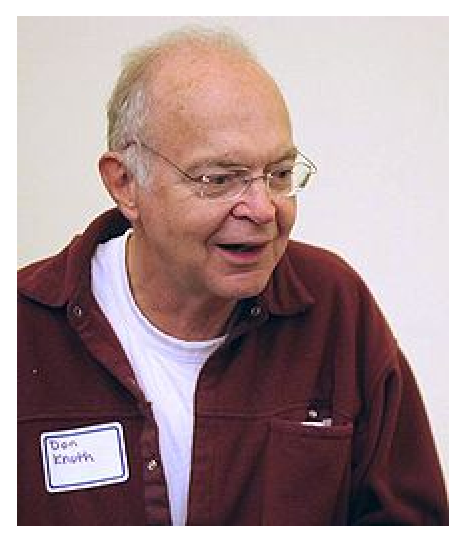
\includegraphics[width=1\linewidth]{knuth1}}
    \end{minipage}
    \hfill
    \begin{minipage}[t]{0.47\linewidth}
        \textbf{Составная \\ подпись 2}
        \center{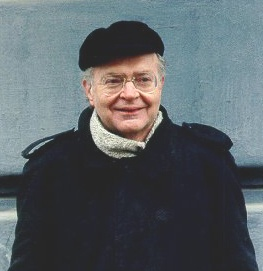
\includegraphics[width=1\linewidth]{knuth2}}
    \end{minipage}
\end{frame}

\subsection{Линии}

\begin{frame}
    \frametitle{Разделяющие линии}
    \begin{minipage}[c]{0.47\linewidth}
        \center{
\includegraphics[width=1\linewidth]{latex}}
        \bigskip
        \hrule{}
        \bigskip
        \textbf{Составная \\ подпись 1}
    \end{minipage}
    \hfill
    \vrule{}
    \hfill
    \begin{minipage}[c]{0.47\linewidth}
        \flushright
        \textbf{Составная \\ подпись 2}
        \center{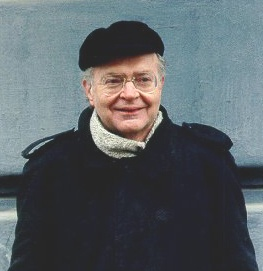
\includegraphics[width=1\linewidth]{knuth2}}
    \end{minipage}
\end{frame}

\section{Остальное}
\begin{frame}[plain, noframenumbering]
    \begin{center}
        \Huge
        Остальное
    \end{center}
\end{frame}

\subsection{Формулы}

\begin{frame}
    \frametitle{Формулы}
    \[
    \left\{
    \begin{array}{rl}
        \dot x = & \sigma (y-x)  \\
        \dot y = & x (r - z) - y \\
        \dot z = & xy - bz
    \end{array}
    \right.
    \]
\end{frame}

\begin{frame}
    \frametitle{amsmath}
    \centering
    \begin{minipage}[t]{0.5\linewidth}
        \begin{multline*}
            y = 1 x^1 + 2 x^2 + 3 x^3 + \\ + 4 x^4 + 5 x^5 + \dots
        \end{multline*}
    \end{minipage}
\end{frame}

\begin{frame}[allowframebreaks]
    \frametitle{Уравнения Максвелла}
    \centering{
        \small
        \def\arraystretch{1.8}%
        \begin{tabular}{ll}
            \toprule
            Интегральная форма                                                                                                                                          & Дифференциальная форма                                                        \\ \midrule
            \(Q_e(t) = \displaystyle\oiint_S \vec D(t) \cdot d\vec{s} = \displaystyle\iiint_V \rho_v(t) dv\)                                                              & \(\nabla \cdot \vec D(t) = \rho_v(t)\)                                          \\
            \(\displaystyle\oiint_S \vec B(t) \cdot d\vec{s} = 0\)                                                                                                        & \(\nabla \cdot \vec B(t) = 0\)                                                  \\
            \(V_{emf}(t) = \displaystyle\oint_L \vec E(t) \cdot d\vec{l}\) = \(- \displaystyle\iint_S \left[\frac{\partial\vec{B}(t)}{\partial t}\right] \cdot d\vec{s}\)   & \(\nabla \times \vec E(t) = - \frac{\partial\vec{B}(t)}{\partial t}\)           \\
            \(I(t) = \displaystyle\oint_L \vec H(t) \cdot d\vec{l} = \displaystyle\iint_S \left[\vec J(t) + \frac{\partial\vec{D}(t)}{\partial t}\right] \cdot d\vec{s}\) & \(\nabla \times \vec H(t) = \vec J(t) + \frac{\partial\vec{D}(t)}{\partial t}\) \\ \midrule
            \(\displaystyle\oiint_S \vec J \cdot d\vec{s} = -\frac{\partial Q_e}{\partial t}\)                                                                            & \(\nabla \cdot \vec J = - \frac{\partial \rho_v}{\partial t}\)                  \\
            \bottomrule
            \multicolumn{2}{c}{\(\vec D(t) = \left[\varepsilon(t)\right] * \vec E(t)\)}                                                                                                                                                                   \\
            \multicolumn{2}{c}{\(\vec B(t) = \left[\mu(t)\right] * \vec H(t)\)}                                                                                                                                                                           \\
        \end{tabular}
    }
    \framebreak

    \hspace{0.05\linewidth}
    \centering{
        \small
        \def\arraystretch{1.8}%
        \begin{tabular}{ll}
            \toprule
            Интегральная форма                                                                                                            & Дифференциальная форма                             \\ \midrule
            \(Q_e = \displaystyle\oiint_S \vec D \cdot d\vec{s} = \displaystyle\iiint_V \rho_v dv\)                                         & \(\nabla \cdot \vec D = \rho_v\)                     \\
            \(\displaystyle\oiint_S \vec B \cdot d\vec{s} = 0\)                                                                             & \(\nabla \cdot \vec B = 0\)                          \\
            \(V_{emf} = \displaystyle\oint_L \vec E \cdot d\vec{l}\) = \(- \displaystyle\iint_S \left[j \omega \vec B\right] \cdot d\vec{s}\) & \(\nabla \times \vec E = - j \omega \vec B\)         \\
            \(I = \displaystyle\oint_L \vec H \cdot d\vec{l} = \displaystyle\iint_S \left[\vec J + j \omega \vec D\right] \cdot d\vec{s}\)  & \(\nabla \times \vec H = \vec J + j \omega \vec{D}\) \\ \midrule
            \(\displaystyle\oiint_S \vec J \cdot d\vec{s} = - j \omega Q_e\)                                                                & \(\nabla \cdot \vec J = - j \omega \rho_v\)          \\
            \bottomrule
            \multicolumn{2}{c}{\(\vec D(t) = \left[\varepsilon\right] \vec E(t)\)}                                                                                                               \\
            \multicolumn{2}{c}{\(\vec B(t) = \left[\mu\right] \vec H(t)\)}                                                                                                                       \\
        \end{tabular}
    }
\end{frame}

\subsection{Таблицы}

\begin{frame}
    \frametitle{Таблица}
    \centering
    \begin{tabular}{|l|l|}
        \hline
        \textbf{Заголовок 1} & \textbf{Заголовок 2} \\
        \hline
        Сумма                & \(b+a\)                \\
        \hline
        Разность             & \(a-b\)                \\
        \hline
        Произведение         & \(a*b\)                \\
        \hline
    \end{tabular}
\end{frame}

\begin{frame}
    \frametitle{Другая таблица}
    \centering
    \begin{tabular}{lc}
        \toprule
        \multicolumn{1}{c}{\textbf{Заголовок 1}} & \textbf{Заголовок 2} \\ \midrule
        Сумма                                    & \(b+a\)                \\
        Разность                                 & \(a-b\)                \\
        Произведение                             & \(a*b\)                \\
        \bottomrule
    \end{tabular}
\end{frame}


\subsection{Разное}

\begin{frame}
    \frametitle{Большой многоуровневый список}
    \begin{itemize}
        \item \textbf{Пункт 1}
              \begin{itemize}
                  \itemi Подпункт 1-1
                  \itemi Подпункт 1-2
              \end{itemize}
        \item \textbf{Пункт 2}
              \begin{itemize}
                  \itemi Подпункт 2-1
              \end{itemize}
        \item \textbf{Пункт 3}
              \begin{itemize}
                  \itemi Подпункт 3-1
                  \itemi Подпункт 3-2
              \end{itemize}
        \item \textbf{Пункт 4}
              \begin{itemize}
                  \itemi Подпункт 4-1
              \end{itemize}
        \item \textbf{Пункт 5}
              \begin{itemize}
                  \itemi Подпункт 5-1
                  \itemi Подпункт 5-2
                  \itemi Подпункт 5-3
              \end{itemize}
    \end{itemize}
\end{frame}

\begin{frame}
    \frametitle{Четыре изображения}
    \centering
    
\includegraphics[width=0.35\linewidth,angle=35]{latex}
    
\includegraphics[width=0.35\linewidth,angle=135]{latex}\\
    
\includegraphics[width=0.35\linewidth,angle=15]{latex}
    
\includegraphics[width=0.35\linewidth,angle=-15]{latex}
\end{frame}

       % Настройки заглавной странице
%\begin{frame}
    \frametitle{Научная новизна}
    \begin{itemize}
  \item {Выявлены закономерности переноса знаний при псевдоразметке данных для многозадачных нейросетевых моделей с одним линейным слоем.}
  \item {Выявлены закономерности переноса знаний в энкодер-агностичных многозадачных нейросетевых моделях между различными диалоговыми задачами и языками. Была получена оценка зависимости этого переноса от размера обучающей выборки. Была проверена также справедливость выводов о межъязыковом переносе для однозадачных моделей.}
  \item {Получена оценка зависимости межъязыкового переноса знаний на разговорных данных в многоязычных нейросетевых моделях от размера предобучающей выборки и генеалогической близости языков к языку дообучения.}
  \item {Разработана диалоговая платформа DREAM и показана ее пригодность для изучения прикладного применения многозадачных нейросетевых моделей.}
  \item {Рассмотренные в диссертации многозадачные нейросетевые архитектуры были интегрированы в диалоговую платформу DREAM, была оценена их применимость и был проведен их сравнительный анализ на основе опыта применения. На основании этого анализа была произведена также интеграция в библиотеку DeepPavlov, находящуюся в открытом доступе.}
    \end{itemize}
\end{frame}
\note{
}

\begin{frame}
    \frametitle{Практическая значимость}
    \begin{itemize}
   \item Впервые в России была создана диалоговая платформа мирового уровня, вышедшая в полуфинал престижных мировых конкурсов Alexa Prize 3 и Alexa Prize 4 (в конкурсах было 10 и 9 участников соответственно, из более чем 300 кандидатов). Эта диалоговая платформа имеет полностью открытый код, что дает возможность легкого переиспользования любой части проделанной над ней работы. Были также разработаны сценарные навыки для этой платформы.
   \item В данной диалоговой платформе были применены многозадачные нейросетевые модели: многозадачная нейросетевая модель с одним линейным слоем, многозадачная нейросетевая модель на основе архитектуры PAL-BERT и многозадачная энкодер-агностичная нейросетевая модель.
   \item Программный код для реализации многозадачной энкодер-агностичной нейросетевой модели встроен в библиотеку DeepPavlov, имеющую более 500000 скачиваний на март 2023 года.
    \end{itemize}
\end{frame}
\note{
}


\iffalse
\begin{frame}
    \frametitle{Акт о внедрении}
    \begin{figure}[h]
        \centering
        \fbox{
            \begin{minipage}[t]{0.4\linewidth}
                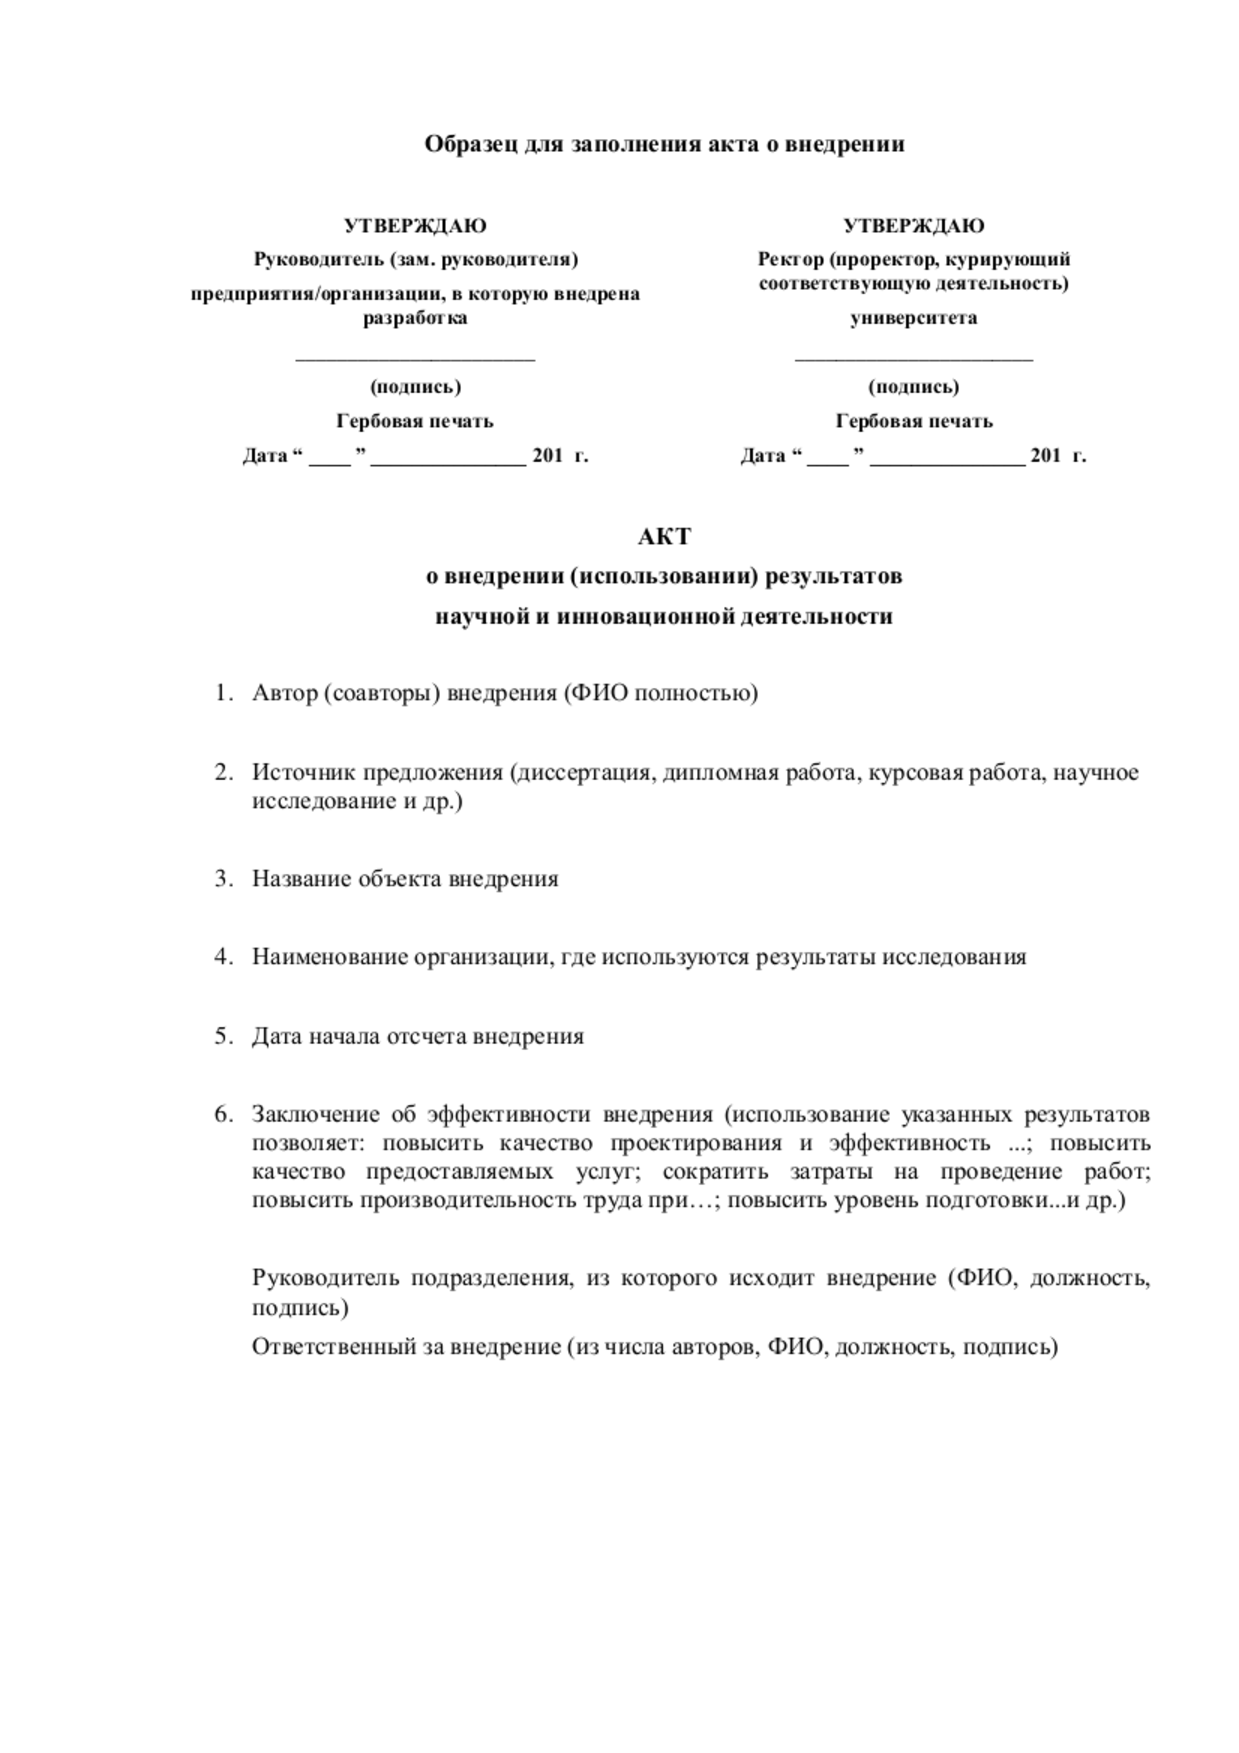
\includegraphics[width=\linewidth]{implementation}
            \end{minipage}
        }
    \end{figure}
\end{frame}
\note{
    Получен акт о внедрении.
}
\fi

% \begin{frame} % публикации на одной странице
\begin{frame}[t,allowframebreaks] % публикации на нескольких страницах
    \frametitle{Основные публикации}
    \nocite{pseudolabel}
    \nocite{rumtl}%
    %\nocite{enmtl}%
    \nocite{rutopics}
    \nocite{dream1}
    \nocite{dream1_trudy}
    \nocite{dream2}
    \nocite{dp_2023}
    \ifnumequal{\value{bibliosel}}{0}{
        \insertbiblioauthor
    }{
        \printbibliography%
    }
\end{frame}
\note{
    Результаты работы опубликованы в N печатных изданиях, в т.ч. M реферируемых изданиях.
}

\begin{frame}
    \frametitle{О результатах доложено на конференциях}
    \begin{itemize}
   \item En\&T 2018, доклад «Разработка диалоговой системы с интеграцией профиля личности», Даниил Болотин, Дмитрий Карпов, Григорий Рашков, Иван Шкурак, 15-16 ноября 2018 года, Москва;
   \item Диалог-2021, доклад «Data pseudo-labeling while adapting BERT for multitask approaches», Dmitry Karpov, Mikhail Burtsev, 16-19 июня 2021 года, Москва;
   \item AINL-2023, доклад «YAQTopics: Russian Conversational Topic Dataset», Dmitry Karpov, Vasily Konovalov, Mikhail Burtsev, 20-22 апреля 2023 года, Ереван, Армения
    \end{itemize}
\end{frame}
\note{
}

\begin{frame}[plain, noframenumbering] % последний слайд без оформления
    \begin{center}
        \Huge
        Спасибо за внимание!
    \end{center}
\end{frame}
    % Последние слайды презентации
%\appendix
%\iffalse
\begin{frame}
    \frametitle{Ответы на замечания ведущей организации ФИЦ ИУ РАН}
    \begin{itemize}
        1. В работе не приведена численная оценка того, насколько сильно псевдоразметка данных улучшает показатели энкодер-агностичной модели.
        ОТВЕТ:
        2. Повсеместно вместо принятых в русскоязычной литературе терминов "мера качества", "индекс качества" или "показатель качества" используется термин "метрика", что является некорректным переводом английского "quality metric".
        ОТВЕТ:
        3. В первых трёх главах нет отдельного раздела "выводы", хотя сами выводы даны.
    \end{itemize}
\end{frame}

\begin{frame}
    \frametitle{Ответы на замечания рецензента Сорокина Артема Юрьевича}
    \begin{itemize}
1. Работе не хватает консистентности и ясности в оформлении таблиц.  В части таблиц жирным выделены лучше полученные на задаче результаты (таб. 3, 5, 22, 23). Часть таблиц с результатами не использует выделения (таб. 4, 8, 19). Часть таблиц игнорирует лучшие результаты в определенных строках, но выделяет их в других (таб. 1, 2). В части таблиц не представляется возможным понять правило, по которому одни значения выделяются жирным, а другие - нет (таб. 26). В сопутствующем тексте и описании таблиц не упоминается использование жирного шрифта для выделения чего-либо.  

1. В большинстве экспериментов в данной работе (например, таблицы 1-8, графики на рисунках 3.1, 3.2) приводится только выборочное среднее по некоторому числу независимых запусков модели.  При этом для этих экспериментов не посчитаны доверительные интервалы или хотя бы значение стандартного отклонения для выборки. Это затрудняет возможность делать выводы о том, как сравниваемые методы действительно соотносятся друг с другом. 
2. Автор работы постоянно обращает внимание на то, что рассматриваемые им многозадачные модели требуют меньше вычислительных ресурсов по сравнению с использованием нескольких однозадачных моделей (стр. 6, 9, 47, 86). Проблема заключается в том, что эти утверждения являются слишком общими и вводят в заблуждение. Например, значительная часть многозадачных моделей, предложенных автором, использует при обучении результаты работы специализированных однозадачных моделей (см. разделы 2.3.5 и 2.3.6). Таким образом, обучение многозадачной модели обязательно потребует больших вычислительных ресурсов, так-как уже включает в себя обучение всех однозадачных моделей. Только ближе к концу диссертации становится понятно, что автор имеет в виду экономию вычислительных ресурсов на стадии применения модели, игнорируя затраты на стадии её обучения. 
    \end{itemize}
\end{frame}

\begin{frame}
    \frametitle{Ответы на замечания рецензента Малых Валентина}
    \begin{itemize}
Работа посвящена только исследованию переноса знаний в моделях, основанных на использовании кодировщиков, например, архитектуре BERT. В работе не проводилось исследование переноса знаний в моделях, использующих декодировщик либо комбинацию кодировщика и декодировщика, например, LLaMA или ChatGPT.
В главе 2 исследование проведено исключительно на англоязычном наборе задач GLUE, в то время как в последующих главах использовались наборы данных на двух языках, русском и английском. 
Также в диссертации был исследован только перенос знаний с английского языка на русский, но, например, не в обратном направлении.
По тексту диссертации используется большое количество калькированных терминов, самый характерный из них - “энкодер-агностичный”. 
    \end{itemize}
\end{frame}

Замечания в рыбе для Казанцева

В разделе "Экономия памяти GPU, CPU и быстродействия" не указано, на каких устройствах проводились измерения.

В статье не указано, насколько хорошо рассмотренная многозадачная энкодер-агностичная модель решает задачи ответа на вопросы, хотя указано, что возможность решения таких задач тоже поддерживается.

Замечания в рыбе для Харламова

В работе не приведены показатели модели с одним линейным слоем на всём наборе данных GLUE.

Замечания в рыбе для Бурнаева

В работе не приведены примеры того, как модель классифицирует конкретные примеры.

В работе не приведены показатели модели PAL-BERT на всём наборе данных GLUE.

Замечания в рыбе для Тюменцева

Выводы о том, какие факторы влияют на перенос знаний, сделаны только на основе русского языка.

На графиках для англоязычных данных в Главе 3 не приведено СКО.

\fi

Лучше функциональные безобидные. орфография оформление формулировки итд.      % Запасные слайды презентации
\end{document}
